\documentclass[11pt]{article}
\usepackage[margin=1in]{geometry}
\usepackage{amsmath,amssymb}
\usepackage{booktabs}
\usepackage{xcolor}
\usepackage{graphicx}
\usepackage{parskip}        % no paragraph indent; separate paragraphs by vertical space
\usepackage{listings}
\usepackage{tikz}
\usetikzlibrary{positioning,arrows.meta,fit,backgrounds,calc,shapes.geometric}
\usepackage[colorlinks=true,linkcolor=blue,urlcolor=blue,citecolor=blue]{hyperref}

\definecolor{cset}{RGB}{31,119,180}
\definecolor{cfield}{RGB}{44,160,44}
\definecolor{cop}{RGB}{214,39,40}
\definecolor{cgray}{RGB}{120,120,120}

\lstdefinestyle{yaml}{
  basicstyle=\ttfamily\scriptsize,
  frame=single,
  backgroundcolor=\color{gray!7},
  columns=fullflexible,
  breaklines=true,
  keepspaces=true,
  showstringspaces=false,
  commentstyle=\color{cgray}\itshape,
  morecomment=[l]{\#},
}

\newcommand{\code}[1]{\texttt{#1}}

\title{\textbf{Plexus}\\[3pt]
\large A blueprint for differentiable tissue}
\author{Janelia Research Campus}
\date{\today}

\begin{document}
\maketitle

\begin{abstract}
The central challenge in computational biology is not parameter optimization but
model discovery. When observations cannot be explained, optimizing existing
parameters often finds compensating solutions rather than revealing the missing
mechanism. Progress therefore requires searching over competing mechanistic
models, not only over parameter values.

We introduce \emph{Plexus}, a formal language for biological modelling built on
a common abstraction of living systems. Plexus is derived by decomposing the
large existing corpus of simulation models---from neural computation
(Hodgkin--Huxley, connectome and neural-network models), multicellular dynamics
(vertex, Cellular Potts and active-matter models), transport processes
(diffusion, chemotaxis and reaction--diffusion), and developmental dynamics
(embryogenesis, morphogenesis and tissue mechanics)---into a common
representation. Every simulation model is expressed through five primitives:
\emph{sets} of biological entities, the \emph{states} carried by each entity,
continuous spatial \emph{fields}, \emph{maps} relating entities across scales,
and \emph{operators} describing their interactions and transformations.
Operators are further organized by the hierarchy of interactions they implement
(set--set, set--field, field--field, and parent--child), allowing heterogeneous
simulation models to be decomposed, recomposed, and extended within a common
language. Every primitive is paired with a differentiable counterpart:
operators become differentiable functions, maps become differentiable
transformations, and fields may be represented explicitly or as neural implicit
representations. Biological models expressed in Plexus can therefore be
optimized end-to-end without sacrificing mechanistic interpretability.

This separation between biological description and numerical
implementation enables a new workflow for scientific discovery. Agentic systems
can first assemble and compare competing mechanistic hypotheses, then optimize
their parameters against experimental observations, using persistent residuals
to identify missing mechanisms and motivate new operators. Plexus therefore
provides a common language in which simulation, inverse modelling, and
hypothesis generation become successive stages of mechanistic model discovery.

\end{abstract}
\end{abstract}

\part*{Part I --- The abstraction}
\addcontentsline{toc}{section}{Part I --- The abstraction}

\section{Two entities: sets and fields}
\label{sec:entities}

The container is built from two kinds of object: \textbf{sets} and \textbf{fields}.
A \textbf{set} $S_k$ is a discrete collection of like elements at one scale ---
particles, cells, populations, organisms, or the compartments inside a cell:
membrane particles, cytoplasm, nuclei, and metabolites (Fig.~\ref{fig:hier}). Every
element of a set shares the same state schema and the same operators, and a set is
stored as batched tensors --- never one object per element.

Sets are linked by \textbf{containment}. A parent map
\[
  \pi : S_k \longrightarrow S_{k+1}
\]
sends each element to the parent that contains it --- a particle to its cell, a
cell to its population. A cell is therefore not a single object but the collection
of everything that maps to it: its particles, nucleus, metabolites, and any other
child sets. Stacked across scales, these maps form the \emph{containment graph} of
the next section.

A \textbf{field} $f:\Omega\to\mathbb{R}^c$ is a continuous quantity defined on its
own grid --- morphogen concentration, pressure, substrate stiffness, or an
extracellular chemical. Fields are \emph{not} part of the containment graph: they
do not contain cells, and cells do not contain fields. Instead, each field is
coupled to one or more sets through \emph{exchange} operators --- secretion,
sensing, particle--grid transfer, or field sampling (Section~\ref{sec:operators}).

\begin{figure}[h]
\centering
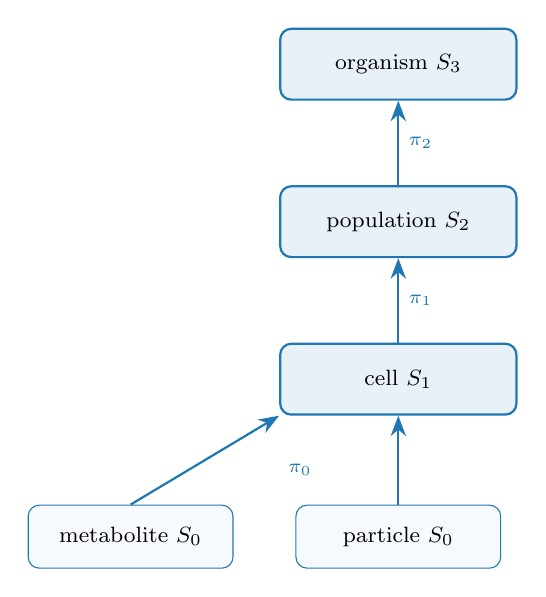
\begin{tikzpicture}[
  font=\footnotesize,
  set/.style={draw=cset,thick,rounded corners,fill=cset!10,minimum width=30mm,minimum height=9mm},
  leaf/.style={draw=cset,rounded corners,fill=cset!4,minimum width=26mm,minimum height=8mm},
  cont/.style={-{Stealth[length=2.6mm]},cset,thick},
]
\node[set] (org)  at (0,6.0) {organism $S_3$};
\node[set] (pop)  at (0,4.0) {population $S_2$};
\node[set] (cell) at (0,2.0) {cell $S_1$};
\node[leaf] (part) at (0,0.0) {particle $S_0$};
\node[leaf] (mol)  at (-3.4,0.0) {metabolite $S_0$};
\draw[cont] (part) -- (cell);
\draw[cont] (mol.north) -- (cell.south west);
\node[cset,font=\scriptsize] at (-1.25,0.85) {$\pi_0$};   % maps both leaves into the cell
\draw[cont] (cell) -- node[right,font=\scriptsize,pos=0.5]{$\pi_1$} (pop);
\draw[cont] (pop)  -- node[right,font=\scriptsize,pos=0.5]{$\pi_2$} (org);
\end{tikzpicture}
\caption{Containment across scales: each parent map $\pi$ sends an element to the
one that contains it. A cell is the collection of everything that maps to it ---
here its particles and metabolites; in general also its membrane, nucleus, and
other child sets (Section~\ref{sec:graph}).}
\label{fig:hier}
\end{figure}

\section{State: what each element carries}
\label{sec:state}

A set says \emph{what exists}; its \textbf{state} says \emph{what each element
carries}. State is a first-class concept, not an implementation detail: every set
declares a typed record of named quantities --- its \emph{state schema} --- and that
record is the sole interface between the set and every operator, plotter, and
integrator that touches it. A particle carries \code{pos}, \code{vel}, and the MPM
continuum blocks \code{F}, \code{C}; a neuron carries \code{voltage}, \code{calcium},
\code{adaptation}; a cell carries \code{polarity}, \code{stiffness}, \code{growth}; a
synapse carries its gating and plastic weight. A field carries state too --- its grid
values --- but the per-element record is what makes the sets interchangeable.

\begin{center}
\footnotesize
\renewcommand{\arraystretch}{1.2}
\begin{tabular}{@{}lll@{}}
\toprule
\textbf{set} & \textbf{state (named blocks)} & \textbf{operators that transform it} \\
\midrule
\code{particle} & \code{pos}, \code{vel}, \code{F}, \code{C}          & MPM strain/scatter/gather, boids \\
\code{neuron}   & \code{voltage}, \code{calcium}, \code{adaptation}   & \code{neuron\_voltage}, \code{signal} \\
\code{cell}     & \code{polarity}, \code{stiffness}, \code{growth}    & division, adhesion, polarity align \\
\code{synapse}  & \code{g} (gating), \code{plastic\_w}                & \code{synapse\_ode} \\
\bottomrule
\end{tabular}
\end{center}

Two consequences make state the pivot of the whole language.

\paragraph{Operators are state $\to$ state.} An operator reads some named blocks of a
set's state and returns a derivative on others --- nothing else.
\code{neuron\_voltage} reads \code{voltage} and the aggregated synaptic current and
returns $d\,\code{voltage}$; \code{mpm\_strain} reads \code{F} and returns its update;
a boid rule reads \code{pos}/\code{vel} and returns an acceleration. Because the
engine integrates whatever block the schema declares dynamical
(Section~\ref{sec:schedule}), a new kind of dynamics is a new state block plus an
operator that returns its derivative --- never an engine change. This is why
\code{pos}/\code{vel} is not privileged: it is simply the state a moving particle
happens to carry.

\paragraph{The frameworks become specifications.} Once state is first-class, the
sibling frameworks stop being separate code and become different \emph{states} over
the same five concepts. connectome-cx is the specification with sets
\code{network}, \code{neuron}, \code{synapse} and operators \code{neuron\_voltage},
\code{synapse\_ode}; an embryogenesis model reuses the identical set machinery with
operators \code{cell\_grow}, \code{active\_stress}, and a cardiac model swaps in
\code{active\_force} --- same language, different vocabulary.
The engine, the maps, and the schedule are identical; only the state schemas and the
operator list change. The whole framework is then five concepts --- \textbf{sets},
\textbf{state}, \textbf{fields}, \textbf{maps}, \textbf{operators} --- and everything
else is a specification written in them.

\paragraph{Anatomy is structure; assemblies are emergent.} Structure stays
anatomical: the neural hierarchy is
\code{network}$\to$\code{region}$\to$\code{column}$\to$\code{neuron}$\to$\code{compartment},
each a set contained in the next. A functional \emph{assembly} is deliberately
\emph{not} a level in this tree --- it is an emergent subset selected by a map or a
state (\code{neuron[active=1]}), computed on demand --- so anatomy and computation
are never conflated inside the containment graph.

\paragraph{Operators are contracts; implementations are backends.} A
state\,$\to$\,state operator is a \emph{contract}, not a piece of biophysics.
\code{neuron\_voltage} is the contract ``membrane state $\to$ its derivative''; its
implementations --- Hodgkin--Huxley, Izhikevich, Morris--Lecar, FitzHugh--Nagumo, a
Neural ODE, an MLP, a Transformer --- are interchangeable, and the spec selects one
without touching the maps, the schedule, or the rest of the model
(\code{\{op: neuron\_voltage, implementation: hodgkin\_huxley\}}). Likewise
\code{synapse\_ode} is a contract with conductance, alpha, plastic, and complex-phase
implementations. The two most developed neural frameworks are then two
\emph{backends} of the \emph{same} contracts, not two engines: \textbf{Jaxley}
implements \code{neuron\_voltage} as multicompartment Hodgkin--Huxley and
\code{synapse\_ode} as a conductance synapse, differentiating through an implicit
solver; a connectome \textbf{GNN} implements the same contracts as learned message
functions, promoting the scalar voltage to a coupled $(v,c)$ state and rotating the
postsynaptic response by a broadcast neuromodulator $\alpha$.

\paragraph{Morphology is Sets, not an embedding.} The two differ only in
\emph{resolution}, and even that is structural. Plexus keeps morphology as multiscale
sets --- \code{neuron}$\to$\code{compartment}$\to$\code{ion\_channel} --- so Jaxley's
explicit compartments are the fine-grained end of the same containment hierarchy and
its channels are operators on the \code{compartment} set. The GNN's geometry
embedding $s_i$ is a \emph{model reduction} of that hierarchy: one implementation that
summarises the compartment tree in a frozen per-neuron feature. Explicit compartments
and a geometry embedding are thus two \emph{resolutions} of one hierarchy, not two
data models --- which is what makes mechanism search well posed: holding the sets,
states, and maps fixed, the search ranges over the implementation of each contract
and the resolution of each hierarchy.

\paragraph{An intermediate representation, not a simulator.} Taken together this is
the thesis of Plexus. It is not another simulator but a typed \emph{intermediate
representation} for biological computation: a model expressed in \textsc{Neuron},
Jaxley, Flyvis, connectome-cx, an embryogenesis solver, or a cardiac model compiles
to the same sets, states, maps, fields, operators, and schedule, and each existing
simulator becomes a \emph{backend} implementing one family of operator contracts.
Plexus is to a biophysics simulator what \textsc{LLVM} is to a C compiler --- the
payoff is portability (one model, many backends) and mechanism search, not a faster
solver.

\section{Maps between sets}
\label{sec:graph}

Section~\ref{sec:entities} named the sets; this section connects them. Sets are
connected by named \textbf{maps}, and there is only one primitive here: a map
$m:S_a\to S_b$ is an index relation sending each element of one set to an element of
another. Hierarchy, connectivity, signalling, transport, and compartmental
organization are all expressed through collections of such maps; the engine
manipulates maps uniformly, and only their biological interpretation differs. This is
the third primitive, on the same footing as sets and fields, and it is what lets the
framework grow without special cases: the container is not $(S,F,\pi)$ --- sets,
fields, and a single hardcoded parent map --- but $(S,F,M)$, sets and fields over an
\emph{open collection of named maps}. An operator names the map it traverses
(\code{via: parent}, \code{via: post}) and never branches on which.

We name a map by the role it plays --- a convention for the reader, not a distinction
the engine makes. A \textbf{parent map} $\pi:S_k\to S_{k+1}$ sends a child to the one
parent that owns it; stacked across scales the parent maps form the hierarchy (an
acyclic tree), and biologists call this relation \emph{containment}. A \textbf{pre}
or \textbf{post map} $\iota:S_e\to S_k$ sends an \emph{edge-entity} (a synapse, a
junction, a vessel segment) to one of its endpoints, so a stateful connection carries
several such maps at once; biologists call this \emph{incidence}. The parent map
builds the tree; pre/post maps overlay a graph on it. We take the parent map first,
since it defines the hierarchy, then pre/post maps, which let recurrent circuits and
other stateful connections live inside that hierarchy without breaking the tree.

\subsection*{The parent map: the hierarchy}

Two points make the parent map precise, and they are what keep the engine free of
branching.

\paragraph{One set per kind of object.} Rather than a single set whose elements
carry a label saying what each one is --- which forces every operator to ask
``what am I looking at?'' at run time --- we keep \emph{one set per kind}: membrane
particles, nuclei, metabolites, and cells are separate sets, each with its own
state schema, operators, and fields. An operator then names the one set it acts on
(\code{at: nucleus}) and never branches. This is the same discipline an
entity--component system or a relational database already uses.

\paragraph{Joined by parent maps.} The sets are joined by parent maps, declared
simply by naming the parent,
\[
  \pi : S_k \longrightarrow S_{k+1},
\]
which send every element to the parent that contains it. A parent may have many
children, so the parent map is a \textbf{graph}, not a chain: one cell gathers several
child sets at once (Fig.~\ref{fig:graph}). The engine needs only two things ---
\code{Level.parent} (which parent each element has) and \code{Level.parent\_name}
(which set that parent belongs to) --- so new biological structure is just a new
set and a parent map, never an engine change.

\paragraph{A new set, or a new type?} The rule (Table~\ref{tab:sorts}): two groups
that differ in \emph{state or operators} are \emph{different sets}; two groups that
share both and differ only in \emph{parameter values} are \emph{types within one
set} --- the \code{types:} block. A cell and a nucleus have different state and
dynamics, so they are different sets; a soft cell and a stiff cell differ only in
stiffness, so they are two types of the single cell set.

\begin{table}[h]
\centering\footnotesize
\renewcommand{\arraystretch}{1.3}
\begin{tabular}{@{}l p{5.1cm} p{5.1cm}@{}}
\toprule
 & \textbf{Different sets} & \textbf{Types within one set} \\
\midrule
example     & membrane vs.\ nucleus vs.\ metabolite      & soft cell vs.\ stiff cell \\
differ in   & state space $+$ operators                  & only parameter values \\
in the spec & separate \code{sets:} with \code{parent:}   & a \code{types:} block inside one set \\
dispatch    & by name (\code{at: nucleus})               & per-element parameter lookup \\
\bottomrule
\end{tabular}
\caption{When to declare a new set versus a new type: a different \emph{kind}
(state space or dynamics) $\Rightarrow$ a new set; a parametric \emph{variant}
$\Rightarrow$ a type within a set.}
\label{tab:sorts}
\end{table}

Keeping each operator attached to its own set is the payoff: \code{membrane\_tension}
acts on \code{membrane\_particle}, \code{metabolism} on \code{metabolite}, and
\code{gene\_regulation} on \code{nucleus}, while Exchange operators connect
compartments explicitly (nucleus\,$\leftrightarrow$\,cytoplasm,
membrane\,$\leftrightarrow$\,extracellular field) --- never one mega-operator
branching on a role flag.

\begin{figure}[h]
\centering
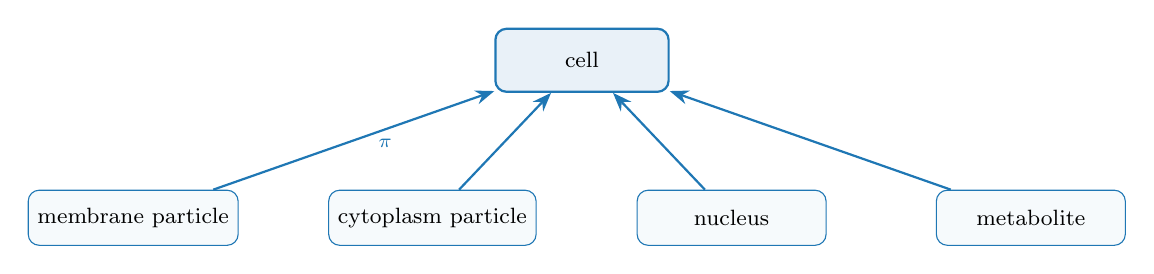
\begin{tikzpicture}[font=\footnotesize,
  set/.style={draw=cset,thick,rounded corners,fill=cset!10,minimum width=22mm,minimum height=8mm},
  leaf/.style={draw=cset,rounded corners,fill=cset!4,minimum width=24mm,minimum height=7mm},
  cont/.style={-{Stealth[length=2.4mm]},cset,thick},
]
\node[set] (cell) at (0,0) {cell};
\node[leaf] (mem) at (-5.7,-2.0) {membrane particle};
\node[leaf] (cyt) at (-1.9,-2.0) {cytoplasm particle};
\node[leaf] (nuc) at (1.9,-2.0) {nucleus};
\node[leaf] (met) at (5.7,-2.0) {metabolite};
\draw[cont] (mem) -- (cell); \draw[cont] (cyt) -- (cell);
\draw[cont] (nuc) -- (cell); \draw[cont] (met) -- (cell);
\node[cset,font=\scriptsize] at (-2.5,-1.05) {$\pi$};
\end{tikzpicture}
\caption{A containment graph: one parent set (\code{cell}) with several child
sets, each with its own parent map. The cell is the collection of these children
--- not a bag of one kind of particle. A new compartment is a new row in the spec
(Listing~\ref{lst:cell}), not an engine edit.}
\label{fig:graph}
\end{figure}

\begin{lstlisting}[style=yaml,caption={A cell as a collection of child sets: each compartment is its own set with a parent map.},label=lst:cell]
sets:
  cell:               {n: 100}
  membrane_particle:  {parent: cell, per_parent: 64,  role: membrane}
  cytoplasm_particle: {parent: cell, per_parent: 200, role: cytoplasm}
  nucleus:            {parent: cell, per_parent: 1,   role: nucleus}
  metabolite:         {parent: cell, per_parent: 50,  role: metabolite}
\end{lstlisting}

\subsection*{Pre and post maps: stateful connections as edge-sets}
\label{sec:incidence}

The parent map is a tree: every element has exactly one parent. But a
\emph{connection} joins two elements and belongs to neither exclusively --- a
chemical synapse has one presynaptic and one postsynaptic neuron, and is owned by
both and by neither. A connection is therefore not a parent map; it is another map
(indeed a pair) on the same sets.

\paragraph{When a relation is enough, and when it is not.} A connection has two
faithful representations, and which one is correct is set by whether the connection
has \emph{state of its own}.
\begin{itemize}\itemsep2pt
\item \textbf{Passive.} If the edge is a fixed scalar --- a synaptic weight
$W_{ij}$, a spring constant --- it is a \textbf{relation} $E\subseteq S_k\times S_k$
with an edge attribute: exactly the \code{Level.edge\_index} of the previous
section, read in place by a Lateral operator (Section~\ref{sec:operators}).
\item \textbf{Dynamical.} If the edge carries its own evolving state --- synaptic
gating and transmitter, short-term facilitation, a plastic weight, a remodelling
adhesion --- then it is promoted to an \textbf{edge-set} $S_e$: a first-class set
whose \emph{elements are the connections}, with their own state schema and their own
operators, joined to the endpoint sets by \textbf{pre and post maps}.
\end{itemize}
This is the rule: \emph{a relation suffices while an edge is passive; when an edge
carries dynamical state it becomes an edge-set with its own pre/post maps.} The
edge-set is not a new layer or a new engine primitive --- it is an ordinary set that
happens to sit on the connections, and it still has a parent (the \code{network}).

\paragraph{Pre and post maps.} An edge-set element points at its endpoints through
one map per endpoint role. For a directed synapse,
\[
  \iota_{\mathrm{pre}}:S_{\mathrm{synapse}}\to S_{\mathrm{neuron}},
  \qquad
  \iota_{\mathrm{post}}:S_{\mathrm{synapse}}\to S_{\mathrm{neuron}},
\]
send each synapse to its presynaptic and postsynaptic neuron. They do not answer
``who owns me'' (the synapse's parent is the \code{network}), they answer ``whom do I
connect.'' Structurally they are index buffers on the edge-set (\code{.pre},
\code{.post}), the exact analogue of \code{.parent} --- so an operator gathers or
scatters along a pre/post map with the same machinery it uses along the parent map,
and the engine gains no special case. The same shape recurs wherever a stateful
connection does: ligand--receptor contacts
($\iota:S_{\mathrm{ligand}}\to S_{\mathrm{receptor}}$), cell--cell junctions
($\iota_1,\iota_2:S_{\mathrm{junction}}\to S_{\mathrm{cell}}$), and vascular segments
($\iota_{\mathrm{from}},\iota_{\mathrm{to}}:S_{\mathrm{seg}}\to S_{\mathrm{node}}$).

\begin{figure}[h]
\centering
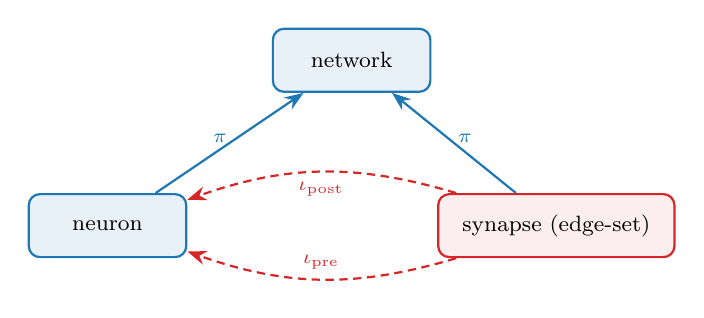
\begin{tikzpicture}[font=\footnotesize,
  set/.style={draw=cset,thick,rounded corners,fill=cset!10,minimum width=20mm,minimum height=8mm},
  edgeset/.style={draw=cop,thick,rounded corners,fill=cop!8,minimum width=30mm,minimum height=8mm},
  cont/.style={-{Stealth[length=2.4mm]},cset,thick},
  inc/.style={-{Stealth[length=2.4mm]},cop,thick,densely dashed},
]
\node[set] (net) at (0,2.1) {network};
\node[set] (neu) at (-3.1,0) {neuron};
\node[edgeset] (syn) at (2.6,0) {synapse (edge-set)};
\draw[cont] (neu) -- node[left,font=\scriptsize,pos=0.55]{$\pi$} (net);
\draw[cont] (syn) -- node[right,font=\scriptsize,pos=0.55]{$\pi$} (net);
\draw[inc] (syn) to[bend left=18] node[above,font=\scriptsize]{$\iota_{\mathrm{pre}}$} (neu);
\draw[inc] (syn) to[bend right=18] node[below,font=\scriptsize]{$\iota_{\mathrm{post}}$} (neu);
\end{tikzpicture}
\caption{The neural hierarchy. Solid \emph{parent} maps $\pi$ (blue) make both
\code{neuron} and \code{synapse} children of the one \code{network} --- the tree.
Dashed \emph{pre}/\emph{post} maps $\iota_{\mathrm{pre}},\iota_{\mathrm{post}}$ (red)
send each synapse edge-entity to the two neurons it connects --- the graph. The
synapse is a set like any other; it merely carries pre/post maps in addition to a
parent.}
\label{fig:neuro}
\end{figure}

\paragraph{Signalling reads off the maps.} Endpoint voltages are \emph{gathered}
onto each synapse along its pre and post maps; the synapse integrates its own state;
its output current, scaled by the synaptic weight $W_e$, is \emph{aggregated} back
onto the postsynaptic neuron; and the neuron integrates its voltage. For synapse $e$
and neuron $i$, writing $\mathrm{pre}(e),\mathrm{post}(e)$ for the maps,
\begin{align*}
\text{synapse (edge-set ODE):}\quad
  & \frac{d s_e}{dt}
    = h\!\big(s_e,\ v_{\mathrm{pre}(e)},\ v_{\mathrm{post}(e)};\ \theta_{\tau(e)}\big),\\[1pt]
\text{synaptic current}\ (\uparrow\ \text{\code{post}}):\quad
  & I_i = \sum_{e:\,\mathrm{post}(e)=i} W_e\, g\big(s_e,\, v_i\big),\\[1pt]
\text{neuron (set ODE):}\quad
  & \tau_i\,\frac{d v_i}{dt}
    = \mathrm{intrinsic}_i(v_i) + I_i + I^{\mathrm{ext}}_i .
\end{align*}
The middle line is an Aggregate (Section~\ref{sec:operators}) run along the
\code{post} map rather than the \code{parent} map: the sum over children of a parent
becomes a sum over the edges into $i$, each weighted by its synaptic weight $W_e$. A
passive connectome is the degenerate case --- drop the synapse state $s_e$, so $g$
collapses to $\phi(v_{\mathrm{pre}(e)})$ and
$I_i=\sum_{e:\,\mathrm{post}(e)=i} W_e\,\phi(v_{\mathrm{pre}(e)})=\sum_j W_{ij}\,\phi(v_j)$,
recovering a single Lateral \code{signal} operator on a plain relation (no edge-set
needed). Listing~\ref{lst:neuro} is the stateful version.

\begin{lstlisting}[style=yaml,caption={A recurrent circuit as one hierarchy: a \code{neuron} set and a \code{synapse} edge-set, both contained in the \code{network}, the synapse joined to the neurons by \code{pre}/\code{post} incidence maps.},label=lst:neuro]
sets:
  network: {n: 1}
  neuron:                                  # an ordinary set
    parent: network
    per_parent: 13731
    types: {T4a: {sign: +1, tau: 0.02}, Mi1: {sign: -1, tau: 0.05}}   # Dale sign, tau
  synapse:                                 # an edge-set: elements ARE the connections
    parent: network                        # containment: owned by the network
    edge_set: true
    pre: neuron                            # incidence iota_pre
    post: neuron                           # incidence iota_post
    state: {g: 0.0, plastic_w: 0.0}        # its own dynamical state
operators:
  - {op: synapse_ode,      at: synapse}                # ds_e/dt = h(s_e, v_pre, v_post)
  - {op: synaptic_current, at: synapse, to: neuron}    # aggregate output onto post neuron
  - {op: neuron_voltage,   at: neuron}                 # tau dv/dt = intrinsic + I_syn + I_ext
schedule: [synapse_ode, synaptic_current, neuron_voltage]
\end{lstlisting}

\section{Operators}
\label{sec:operators}

A GNN is an \textbf{operator} $\mathcal{O}$: a map on \textbf{state}
(Section~\ref{sec:state}) dispatched by the relation it acts on --- it reads named
blocks of a set's state and returns a derivative on others. Equivalently, an operator
changes exactly one of the three things the container holds
(Fig.~\ref{fig:ops}): the \textbf{state} on the nodes, the \textbf{relations}
between them, or the \textbf{entities} themselves. \textbf{Four dynamics operators}
move \emph{state} along a fixed structure, one per relation the container admits,
each returning a time-derivative contribution. \textbf{Rewire} changes the
\emph{relations} --- the edge set $E$, which nodes interact. \textbf{Divide} and
\textbf{Die} change the \emph{entities} --- the node set $|S_k|$, which nodes
exist. Those last three return no state delta. The four dynamics operators:
\begin{align*}
\textbf{Lateral}\quad   & \mathcal{O}_E,\ E\subseteq S_k\times S_k
  &&\text{(ODE interaction $+$ graph Laplacian)}\\
\textbf{Aggregate}\ \uparrow\quad & \textstyle\sum_{m}: S_a \to S_b
  &&\text{(reduction along a map $m$)}\\
\textbf{Broadcast}\ \downarrow\quad & m^{*}: S_b\to S_a
  &&\text{(lift along a map $m$)}\\
\textbf{Exchange}\quad  & \mathcal{S},\mathcal{G}: S_k \leftrightarrow F
  &&\text{(a map to/from a field)}
\end{align*}

\noindent Two pieces of notation: $S_k\times S_k$ is the set of all node \emph{pairs}, so an
edge set $E\subseteq S_k\times S_k$ is simply a graph on $S_k$ --- which nodes
interact (e.g.\ neighbours within a cutoff radius, or a fixed connectome). And
$\mathcal{S},\mathcal{G}$ are the two halves of a field coupling: \emph{scatter}
$\mathcal{S}:S_k\to F$ writes object state into the field, while \emph{gather}
$\mathcal{G}:F\to S_k$ reads it back. Each operator in turn:

\paragraph{Lateral $\mathcal{O}_E$.} Message passing \emph{within} one scale along
the edges $E$. It carries the within-scale physics: pairwise interactions (forces,
adhesion, signalling) plus a graph Laplacian that diffuses or smooths quantities
over the edges. Examples: particle--particle elasticity, cell--cell flocking or
adhesion, neuron--neuron signal propagation.

\paragraph{Aggregate $\textstyle\sum_m$ (up).} Reduces along a map $m$: pools the
elements that $m$ sends to each target into one quantity. Along the \code{parent}
map a cell's position is the mean of its particles, its metabolic state the sum over
its molecules; along the \code{post} map the current into a neuron is the sum over
its incoming synapses (the middle equation of Section~\ref{sec:incidence}). Same
operator, different map named by \code{via:}.

\paragraph{Broadcast $m^{*}$ (down).} The adjoint of Aggregate: it lifts a target's
state back onto every element the map $m$ sends to it. Along the \code{parent} map a
decision taken at the cell level (a body force, a polarity, a signalling output) is
applied identically to all of that cell's particles; along the \code{pre}/\code{post}
maps it gathers the endpoint voltages a synapse needs. Aggregate and Broadcast are a
matched up/down pair on \emph{any} named map, so no new operator is needed for a
stateful connection: \code{synapse\_ode} (a Lateral operator on the synapse edge-set)
sits between a Broadcast that gathers $v_{\mathrm{pre}},v_{\mathrm{post}}$ and an
Aggregate that scatters the current onto the post neuron, and a passive connectome
collapses the whole thing to a single Lateral \code{signal} operator on a plain
relation.

\paragraph{Exchange $\mathcal{S},\mathcal{G}$.} A map whose other endpoint is a
\emph{field} rather than a set: scatter $\mathcal{S}$ deposits/secretes object state
into the field, gather $\mathcal{G}$ samples/senses the field back onto the objects.
It is exactly the MPM particle--grid transfer (P2G/G2P) and chemotactic
secretion/sensing --- Aggregate/Broadcast read as ``set to field / field to set,''
which is why Exchange is not a separate idea so much as the field-valued corner of
the same map primitive.

\paragraph{Rewire $\mathcal{R}$ (relations).} Rewire changes the \emph{relation}
$E\subseteq S_k\times S_k$ on which the lateral operators act --- \emph{which}
nodes are neighbours --- and returns no state delta. A \emph{geometric} relation is
rebuilt every tick from the live configuration (a \textbf{radius graph}: all pairs
within a cutoff; or a $k$-nearest-neighbour or Delaunay graph), so the interaction
graph tracks motion, growth, and division; a \emph{fixed} relation (a connectome)
is built once and never rewired. Rewire is of a different nature from the other
five: it neither moves state nor changes who exists --- it maintains the
\emph{scaffold} the dynamics run on. Separating \emph{who} interacts (Rewire) from
\emph{how} they interact (Lateral) is also what turns a dense $O(N^2)$ force law
into $O(|E|)$ message passing and lets several lateral operators share one graph.

\paragraph{Divide and Die (entities).} The dynamics operators move \emph{state}
and Rewire moves \emph{relations}, both while the node set stays fixed; living
matter also rewrites its own membership. \textbf{Divide}
$\mathcal{B}: x \mapsto \{x',x''\}$ (proliferation) and \textbf{Die}
$\mathcal{D}: x \mapsto \varnothing$ (apoptosis / efflux) are the only operators
that change the \emph{entities} themselves --- the cardinality $|S_k|$. For a
\emph{living} system they are as primordial as the four dynamics operators: a
tissue is defined as much by the cells it makes and loses as by how they move.
Everything else assumes the cells it acts on already exist.

\begin{figure}[h]
\centering
\resizebox{\textwidth}{!}{%
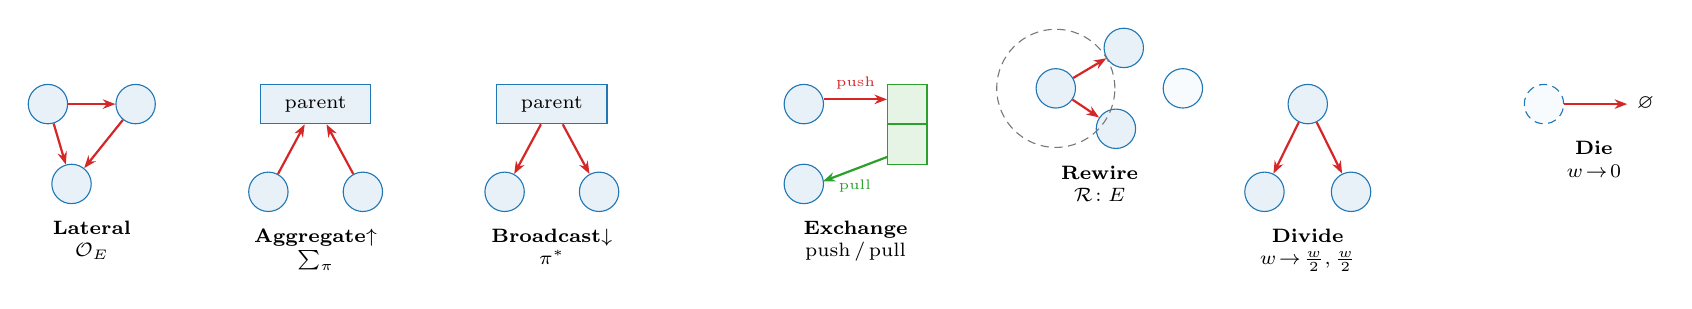
\begin{tikzpicture}[
  font=\scriptsize,
  n/.style={circle,draw=cset,fill=cset!10,minimum size=5mm,inner sep=0},
  p/.style={rectangle,draw=cset,fill=cset!10,minimum width=14mm,minimum height=5mm},
  g/.style={rectangle,draw=cfield,fill=cfield!12,minimum width=5mm,minimum height=5mm},
  a/.style={-{Stealth[length=1.6mm]},cop,thick},
]
\begin{scope}[local bounding box=L]
  \node[n] (a1){}; \node[n,right=6mm of a1](a2){}; \node[n,below=5mm of a1,xshift=3mm](a3){};
  \draw[a] (a1)--(a2); \draw[a] (a1)--(a3); \draw[a] (a2)--(a3);
\end{scope}
\node[below=1mm of L,align=center]{\textbf{Lateral}\\$\mathcal{O}_E$};
\begin{scope}[shift={(34mm,0)},local bounding box=A]
  \node[p] (par){parent};
  \node[n,below=6mm of par,xshift=-6mm](c1){}; \node[n,below=6mm of par,xshift=6mm](c2){};
  \draw[a] (c1)--(par); \draw[a] (c2)--(par);
\end{scope}
\node[below=1mm of A,align=center]{\textbf{Aggregate}$\uparrow$\\$\sum_\pi$};
\begin{scope}[shift={(64mm,0)},local bounding box=B]
  \node[p] (par2){parent};
  \node[n,below=6mm of par2,xshift=-6mm](d1){}; \node[n,below=6mm of par2,xshift=6mm](d2){};
  \draw[a] (par2)--(d1); \draw[a] (par2)--(d2);
\end{scope}
\node[below=1mm of B,align=center]{\textbf{Broadcast}$\downarrow$\\$\pi^*$};
\begin{scope}[shift={(96mm,0)},local bounding box=E]
  \node[n] (o1){}; \node[n,below=5mm of o1](o2){};
  \node[g,right=8mm of o1](g1){}; \node[g,below=0mm of g1](g2){};
  \draw[a,transform canvas={yshift=0.6mm}] (o1)-- node[above,font=\tiny]{push}(g1);
  \draw[a,cfield,transform canvas={yshift=-0.6mm}] (g2)-- node[below,font=\tiny]{pull}(o2);
\end{scope}
\node[below=1mm of E,align=center]{\textbf{Exchange}\\push\,/\,pull};
% --- structure operators (rewire the edges E, change the node set |S|) ---
\begin{scope}[shift={(128mm,2mm)},local bounding box=RW]
  \node[n] (rc){};
  \node[n,above right=1.5mm and 5mm of rc](rn1){};
  \node[n,below right=1.5mm and 4mm of rc](rn2){};
  \node[n,right=11mm of rc,fill=cset!3](rn3){};
  \draw[densely dashed,cgray] (rc) circle (7.5mm);
  \draw[a] (rc)--(rn1); \draw[a] (rc)--(rn2);
\end{scope}
\node[below=1mm of RW,align=center]{\textbf{Rewire}\\$\mathcal{R}\!:E$};
\begin{scope}[shift={(160mm,0)},local bounding box=DV]
  \node[n] (m){};
  \node[n,below=6mm of m,xshift=-5.5mm](g3){}; \node[n,below=6mm of m,xshift=5.5mm](g4){};
  \draw[a] (m)--(g3); \draw[a] (m)--(g4);
\end{scope}
\node[below=1mm of DV,align=center]{\textbf{Divide}\\$w\!\to\!\tfrac{w}{2},\tfrac{w}{2}$};
\begin{scope}[shift={(190mm,0)},local bounding box=DE]
  \node[n,densely dashed,fill=cset!3] (z){};
  \node[right=8mm of z] (nul) {$\varnothing$};
  \draw[a] (z)--(nul);
\end{scope}
\node[below=1mm of DE,align=center]{\textbf{Die}\\$w\!\to\!0$};
\end{tikzpicture}}
\caption{The operators, grouped by what they change. The first four are
\emph{dynamics}: they move \emph{state} along a fixed structure --- \emph{Lateral}
within a set; \emph{Aggregate}/\emph{Broadcast} along a map (the parent map $\pi$, or a \code{pre}/\code{post} map);
\emph{Exchange} to/from a field (P2G/G2P and the metabolite--reaction graph are
both Exchange). The last three return no state delta: \emph{Rewire} changes the
\emph{relations} --- the edge set $E$, which nodes interact (a radius graph rebuilt
each tick, dashed cutoff); \emph{Divide} and \emph{Die} change the \emph{entities}
--- the node set $|S_k|$, cell division and death on a fixed buffer with
per-element occupancy $w$.}
\label{fig:ops}
\end{figure}

\paragraph{Differentiating division and death.} Changing $|S_k|$ is the one move
that resists automatic differentiation: it alters a tensor's shape, and ``does
this cell divide?'' is a discrete event with no useful gradient. We keep the
framework differentiable with a \textbf{continuous-occupancy} formulation. Rather
than resize, we hold a fixed buffer of $N_{\max}$ slots and give every element a
\emph{mass} $w_i\in[0,1]$: \code{Die} decays $w_i\!\to\!0$ (the slot goes
dormant, not deleted); \code{Divide} activates a dormant slot, copies the
mother's state with a small perturbation, and splits the mass
$w\!\to\!(\tfrac{w}{2},\tfrac{w}{2})$. \emph{Every operator then honours $w$}:
Aggregate becomes a \emph{mass-weighted} reduction
$\big(\sum_i w_i x_i\big)/\sum_i w_i$, Lateral weights each message by $w_j$, and
so on --- so the boolean selector mask of Section~\ref{sec:language} is just the
$\{0,1\}$ special case of $w$. The trajectory between events is now smooth in
$w$, so gradients flow on a fixed-shape tensor (and \code{torch.compile} still
applies). The one genuinely non-differentiable part --- the integer decision of
\emph{when} to divide or die --- is handled separately: a straight-through or
Gumbel estimator to learn a division \emph{policy}, a score-function (REINFORCE)
gradient for an expected objective with respect to division/death \emph{rates},
or black-box search (UCB/CEM) when the objective is itself discrete (final count,
fraction escaped). This is the \emph{use both} recipe of Part~III applied to
structure: gradients for the continuous interior, black-box for the discrete
choices.

\section{Dynamics: a schedule}
\label{sec:schedule}

A simulation is a multi-rate composition of operators, declared as a
\code{Schedule}. In math terms, one tick is the composition
$\Phi=\mathcal{O}_n\circ\cdots\circ\mathcal{O}_1$, and the dynamics is its
iteration $x_{t+1}=\Phi(x_t)$ --- a discrete flow. \emph{Multi-rate} means the
operators need not all fire on every tick: a slow process (diffusion, cell
division) can be scheduled to act once every $k$ ticks, while a fast one
(mechanics) runs every tick, so a single \code{Schedule} interleaves dynamics
that evolve on different time scales. The \code{Schedule} is just the code-level
encoding of that composition. Each operator is \emph{pure}: instead of
editing the state in place, it only \emph{returns its contribution} --- a delta
$\Delta_i$ (a time-derivative term) for the sets it touches. The schedule sums the
deltas acting on each set and integrates once per tick.

An operator declares the \emph{order} of its delta, since a time-derivative can be
of position or of velocity. A \emph{first-order} (overdamped) operator returns a
velocity and integrates as $x_{t+1}=x_t+\Delta t\sum_i\Delta_i$; a
\emph{second-order} (inertial) operator returns an acceleration and integrates as
$v_{t+1}=v_t+\Delta t\sum_i\Delta_i,\ x_{t+1}=x_t+\Delta t\,v_{t+1}$. The order is
a fixed property of each operator (\code{EMIT}: \code{velocity} for first order,
\code{acceleration} for second): attraction--repulsion is first order, boids flocking
is second; all engine-integrated operators acting on one set must agree, so the set
integrates as a single order. (A dynamics operator may instead declare \code{EMIT} $=$
\code{mpm\_acceleration} --- an acceleration consumed by the MPM substep as the external
force $a_\text{ext}$ rather than integrated by the engine.) Friction in the inertial case
is itself an operator (a \code{drag} delta $-\kappa v$), not a special term in the integrator.

\paragraph{The integrated quantity is the set's declared state.} Position and
velocity are only the \emph{spatial} instance of this rule. What the engine
integrates is whatever block a set's \emph{state schema} declares dynamical
(Section~\ref{sec:language}): a moving particle declares \code{pos}/\code{vel}, but a
neuron declares a scalar voltage, a metabolite a concentration, a gene its expression
level, a synapse its gating and plastic weight. Each integrates under the same
first-order rule $x_{t+1}=x_t+\Delta t\sum_i\Delta_i$ with $x$ the declared state,
and only the spatial blocks are subject to the world boundary. Making integration
\emph{schema-driven} rather than pos/vel-specific is the single change that lets one
engine carry mechanics, signalling, metabolism, and gene expression at once --- the
temporal counterpart of generalizing a lone hardcoded parent map to the open map
collection $M$. Voltage, calcium, receptor occupancy, and a plastic weight are then
all first-class integrands, each just a schema block plus an operator that returns
its derivative.

Two consequences follow: several operators may
act on the same set in one tick (their deltas simply add --- none overwrites
another), and because nothing is mutated in place, gradients flow through the sums
and the integrator, so the whole rollout stays differentiable. The LLM searches over
schedules and operator parameterizations --- one well-defined action space instead
of per-domain code.

\part*{Part II --- A formal intermediate representation}
\addcontentsline{toc}{section}{Part II --- A formal intermediate representation}

\section{Two layers and the contract between them}

The contribution of this part is not that a language model can drive the
framework --- it is that there is a \textbf{formal intermediate representation}
for anything to drive at all. Between a person's \emph{intent} and a running
\emph{simulation} we interpose one typed, declarative artifact, the \textbf{spec},
and the system becomes a compiler stack:
\[
\text{Intent}\ \longrightarrow\ \text{Language}\ \longrightarrow\ \text{Calculus}\ \longrightarrow\ \text{Simulation}.
\]
Intent compiles to the \textbf{language} (the spec, \code{spec.yaml}); the spec
names primitives in a \textbf{calculus} of operators (the registry); the engine
\textbf{interprets} that calculus into a simulation. In one line: the spec is the
\emph{source}, the registered operators are the \emph{primitives}, and the engine
is the \emph{interpreter}. A language model is one front end on the first arrow ---
useful, but replaceable; the durable object is the representation in the middle.
Every property claimed below is a property of \emph{it}, not of the model that
writes it.

\begin{center}
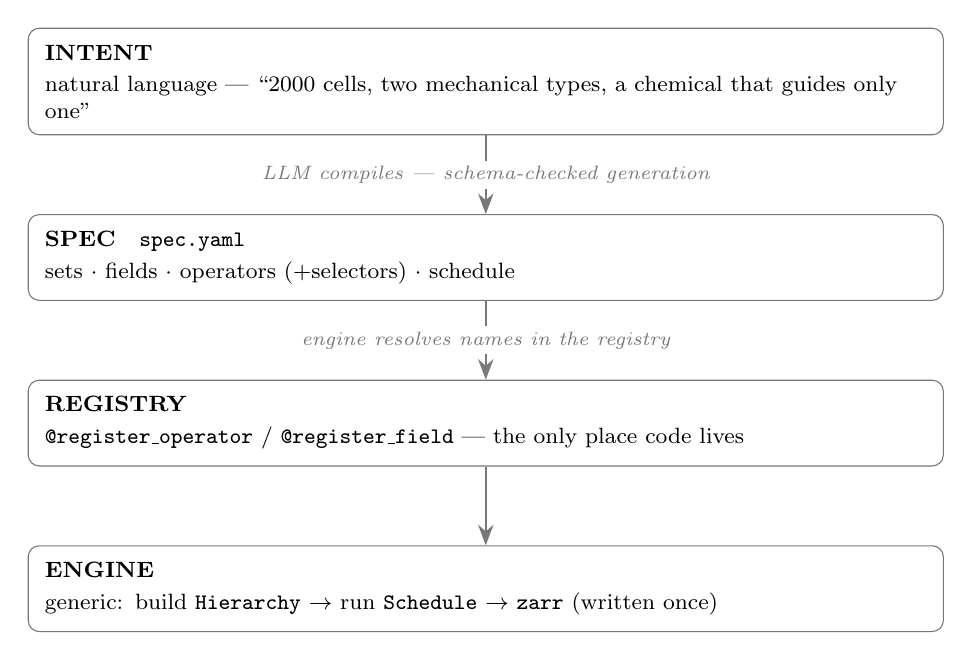
\begin{tikzpicture}[font=\footnotesize,
  layer/.style={draw=cgray,rounded corners,align=left,text width=11.2cm,inner sep=6pt},
  flow/.style={-{Stealth[length=2.6mm]},thick,cgray},
  ann/.style={font=\scriptsize\itshape,fill=white,inner sep=2pt},
]
\node[layer] (intent) {\textbf{INTENT}\\[2pt]natural language --- ``2000 cells, two mechanical types, a chemical that guides only one''};
\node[layer,below=10mm of intent] (spec) {\textbf{SPEC}\quad\code{spec.yaml}\\[2pt]sets $\cdot$ fields $\cdot$ operators ($+$selectors) $\cdot$ schedule};
\node[layer,below=10mm of spec] (reg) {\textbf{REGISTRY}\\[2pt]\code{@register\_operator} / \code{@register\_field} --- the only place code lives};
\node[layer,below=10mm of reg] (eng) {\textbf{ENGINE}\\[2pt]generic: build \code{Hierarchy} $\to$ run \code{Schedule} $\to$ \code{zarr} (written once)};
\draw[flow] (intent) -- node[ann]{LLM compiles --- schema-checked generation} (spec);
\draw[flow] (spec) -- node[ann]{engine resolves names in the registry} (reg);
\draw[flow] (reg) -- (eng);
\end{tikzpicture}
\end{center}

The \textbf{spec is the contract}. The LLM owns everything above it (intent $\to$
spec); the code owns everything below (operators). They never touch directly. This
makes the system both LLM-drivable and human-auditable: the spec is small, typed,
and reviewable, unlike the 500-line flat \code{config.py} it replaces.

Being a small, typed, declarative file gives the contract the properties one wants
of an interface between an unreliable generator and exacting code:
\begin{itemize}\itemsep2pt
\item \textbf{Verifiable.} The spec is validated against the schema \emph{before}
anything runs: an unregistered operator, a missing required property, or a
malformed selector is rejected up front, so a spec that loads is guaranteed
runnable (the missing-operator and missing-property cases below). Beyond
well-formedness, each simulation also ships an \emph{intent} check that measures
whether the requested behaviour actually occurred --- ``it ran'' is not ``it worked''.
\item \textbf{Reproducible.} A run is bit-deterministic given $(\text{spec},
\text{seed})$ --- the engine forces deterministic kernels --- so the same spec
yields the same trajectory, and a fresh seed draws a new realization of the same
dynamics.
\item \textbf{Saveable.} The spec is $\sim$20 lines, so it version-controls, diffs,
and archives trivially; together with the seed it \emph{is} the complete record. We
archive the recipe, not the dish: store spec\,$+$\,seed (plus metrics and a
thumbnail) and regenerate the trajectory on demand (\code{archive.py},
\code{GALLERY.md}).
\item \textbf{Composable.} A variant is a base spec plus a handful of overrides,
which makes ablations and the optimizer's parameter sweeps cheap.
\item \textbf{Extensible.} New behaviour is one new registered operator; the
operator vocabulary grows monotonically, and every earlier spec keeps working.
\end{itemize}

\section{The simulation language}
\label{sec:language}

The contract above is, in effect, a small \textbf{domain-specific language} in
declarative-data form. Like any language it has \emph{words} (vocabulary),
\emph{grammar} (how they combine --- here a typed schema, which \emph{is} the
language definition: required keys, type fractions summing to one, every operator
registered, every schedule token resolving), and \emph{semantics} (what running
them means: the engine builds the \code{Hierarchy} and iterates the schedule,
$x_{t+1}=\Phi(x_t)$). Table~\ref{tab:lang} is the complete vocabulary; every
construct in it appears in the example of Listing~\ref{lst:agg}.

\begin{table}[h]
\centering\footnotesize
\renewcommand{\arraystretch}{1.15}
\begin{tabular}{@{}l p{5.6cm} l@{}}
\toprule
\textbf{Construct} & \textbf{Semantics} & \textbf{Example} \\
\midrule
\multicolumn{3}{@{}l}{\code{general:} --- the run and the world (the space + the clock)}\\
\code{name}        & run identifier                                  & \code{name: aggregate}\\
\code{seed}        & RNG seed --- fixes determinism                  & \code{seed: 0}\\
\code{n\_frames}, \code{dt} & ticks to run; the time step             & \code{n\_frames: 250}\\
\code{boundary}    & the space: \code{periodic} (torus) or \code{wall} (clamp) & \code{boundary: periodic}\\
\code{world}       & domain width $W$; world is $[0,W]\!\times\![0,1]$ ($W{>}1$ longitudinal) & \code{world: 4.0}\\
\code{obstacles}   & static walls (rects or \code{[cx,cy,r]} circles); a BC for the MPM grid $+$ field diffusion & \code{[[.3,0,.36,.7]]}\\
\midrule
\multicolumn{3}{@{}l}{\emph{Set} ($S_k$ --- an entity level / ECS entity)}\\
\code{n}           & size of a top-level set                         & \code{n: 100}\\
\code{parent}      & the set that contains this one --- a containment edge $\pi_{A\to B}$ (many sets may share a parent) & \code{parent: cell}\\
\code{per\_parent} & children per parent                             & \code{per\_parent: 100}\\
\code{role}        & this set's role inside its parent (membrane / cytoplasm / nucleus...) & \code{role: membrane}\\
\code{types}       & named sub-populations: fraction $+$ per-type properties & \code{\{soft: \{fraction: .5, youngs: 12\}\}}\\
\midrule
\multicolumn{3}{@{}l}{\emph{Field} (a continuum)}\\
\code{frame}       & discretization (a grid)                         & \code{frame: grid}\\
\code{res}         & grid resolution                                 & \code{res: 96}\\
\code{diffusion}, \code{decay} & PDE coefficients                    & \code{diffusion: 0.1}\\
\code{couples\_to} & the one set this field exchanges with           & \code{couples\_to: cell}\\
\code{source}      & fixed source region (imposes a gradient)        & \code{source: [.82,.82,1,1]}\\
\code{init}        & uniform initial fill (self-generated runs)      & \code{init: 1.0}\\
\code{navigation}  & \code{geodesic} (precomputed external gradient) or \code{dynamic} (self-generated) & \code{navigation: geodesic}\\
\midrule
\multicolumn{3}{@{}l}{\emph{Operator} (a system; one per list entry)}\\
\code{op}          & which registered operator (contract) to run     & \code{op: sense}\\
\code{implementation} & which \emph{implementation} of that contract to run (default: the only one) & \code{hodgkin\_huxley}\\
\code{at}          & selector --- the subset it acts on              & \code{at: cell[type=soft]}\\
\code{to}/\code{from} & field an Exchange writes to / reads from      & \code{from: chemical}\\
$\langle$params$\rangle$ & operator-specific arguments               & \code{gain: 150}\\
\midrule
\multicolumn{3}{@{}l}{\emph{Selector} (sub-grammar)}\\
\code{set}            & every node of the set                        & \code{cell}\\
\code{set[attr=val]}  & nodes matching \code{attr} (re-checked each tick) & \code{cell[loaded=1]}\\
\midrule
\multicolumn{3}{@{}l}{\emph{Schedule} (sub-grammar; per-tick order)}\\
operator name         & run that operator this tick                  & \code{sense}\\
\code{[a, b]}         & a group run in the same stage                & \code{[glide, sense]}\\
\code{aggregate}      & a registered op: Aggregate$\uparrow$ (parent $=$ mean of children) & \code{aggregate}\\
\code{diffuse}        & a field op: advance that field one step (Laplacian) & \code{diffuse}\\
\midrule
\multicolumn{3}{@{}l}{\code{plotting:} (render style only --- never affects dynamics)}\\
\code{colormap}, \code{point\_size}, \code{background} & how the sets are drawn & \code{background: black}\\
\bottomrule
\end{tabular}
\caption{The simulation language. Each block has its own home in
the spec: \code{general:} is the world and clock,
\code{sets:} are the entities, \code{operators:} the dynamics, \code{schedule:}
the composition, \code{plotting:} the style. Integration is implicit (each set is
integrated once at the end of a tick), so there is no \code{integrate} token.}
\label{tab:lang}
\end{table}

Structurally this is an \textbf{entity--component--system} (ECS) architecture: sets
are entities, their state buffers are components, operators are systems, and the
schedule is the ECS system pipeline. We adopt that framing deliberately --- it is
the cleanest mental model and matches the engine one-to-one. Each entity kind
declares its component layout once in the registry (\code{@register\_entity}): a
typed \emph{state schema} naming which state columns are position, velocity, and
so on, plus \emph{render} hints (what to colour by, whether to draw orientation).
The engine, the operators, and the visualizer all read column semantics from this
one declaration rather than hard-coding offsets like \code{state[:, :2]} ---
so a new entity is drawn and integrated correctly for free.

Most of the spec is plain typed key--value; the only genuine sub-grammars are the
last two blocks of Table~\ref{tab:lang} --- \emph{selectors} and the
\emph{schedule}. Both are deliberately minimal but extend naturally: selectors to
conjunctions and to geometric or temporal predicates (\code{cell[type=soft \& loaded=0]},
\code{cell[x<0.5]}, \code{cell[age>10]}), and the schedule to explicit per-operator
rates and nested loops.

We keep the language as \emph{declarative data} (YAML/JSON) rather than a bespoke
syntax, so an LLM can emit it under schema-constrained decoding and a human can
diff, review, and archive it; the grammar is pinned by a typed schema (Pydantic or
JSON-Schema), and composition, overrides, and parameter sweeps (variants, ablations,
the optimizer) are delegated to a config layer such as Hydra rather than reinvented.
Prior art worth borrowing: ECS engines (the scheduling model), SBML/Antimony
(reaction--species vocabulary), NeuroML and MorpheusML/PhysiCell (multicellular
specs), UFL (PDE operators), and NetLogo/Mesa (agent rules).

A complete spec is a single \code{spec.yaml}. Listing~\ref{lst:agg} assembles the
vocabulary of Table~\ref{tab:lang} into one: two cell \code{types},
\code{particle}s contained in each \code{cell}, one chemical \code{field}, and a
\code{schedule}. Soft cells \code{deposit} the chemical and \code{chemotax} (climb)
it, so they self-aggregate, while stiff cells --- selected out by
\code{cell[type=soft]} --- do not.

\begin{lstlisting}[style=yaml,caption={A complete simulation: soft cells secrete and follow a chemical and self-aggregate.},label=lst:agg]
general: {name: aggregate, seed: 0, n_frames: 250, dt: 0.05, boundary: periodic}
sets:
  cell:
    n: 100
    types: {soft: {fraction: 0.5, youngs: 12}, stiff: {fraction: 0.5, youngs: 300}}
  particle: {parent: cell, per_parent: 100, radius: 0.02}   # containment
fields:
  chemical: {frame: grid, res: 96, couples_to: cell}
operators:
  - {op: glide, at: cell, speed: 15.0, rot: 0.4}
  - {op: mls_mpm_mechanics, at: particle, n_grid: 128, substeps: 8, a_max: 800, drag: 4}
  - {op: deposit,  at: "cell[type=soft]", to: chemical, rate: 1.0}    # only pop 1 makes it
  - {op: diffuse,  at: chemical, rate: 0.1}                           # field self-dynamics (was chemical.diffuse)
  - {op: decay,    at: chemical, rate: 0.05}
  - {op: chemotax, at: "cell[type=soft]", from: chemical, gain: 150.0} # only pop 1 climbs it
schedule: [aggregate, [glide], deposit, diffuse, decay, chemotax, mls_mpm_mechanics]
\end{lstlisting}

The validator (prototype: \code{scenario\_schema.py}) guarantees that a file which
loads is runnable: every \code{op} exists; every \code{at}/\code{to}/\code{from}
references a declared set/field; type \code{fraction}s sum to one; every schedule
token resolves. (One trap: never use a YAML~1.1 boolean key such as
\code{on}/\code{off} --- we use \code{at}.)

\section{Operator catalog}

Operators are the system's vocabulary; it grows monotonically and every past spec
keeps working. The catalog, grouped by what each operator changes (Section~\ref{sec:operators}).
\code{EMIT} is the temporal-integration state a dynamics operator's returned delta
represents --- \code{velocity} / \code{acceleration} integrated by the engine,
\code{mpm\_acceleration} routed to the MPM substep, or \code{---} for an operator that
writes a field, a relation, or a \code{heading} and returns no set delta:

\begin{center}
\renewcommand{\arraystretch}{1.05}
\footnotesize
\resizebox{\textwidth}{!}{%
\begin{tabular}{@{}lll p{6.4cm}@{}}
\toprule
\textbf{op} & \textbf{kind} & \textbf{EMIT} & \textbf{behaviour} \\
\midrule
\multicolumn{4}{@{}l}{\emph{Dynamics --- move a set's state (return a delta)}}\\
\code{signal}                & lateral & velocity & passive connectome: $dv_i=(-v_i+b_i+\sum_j W_{ij}\phi(v_j)+I_i)/\tau_i$ \\
\code{synapse\_ode}          & lateral & velocity & edge-set synaptic state $ds_e/dt=h(s_e,v_{\mathrm{pre}},v_{\mathrm{post}})$ (gathers endpoints along $\iota$) \\
\code{synaptic\_current}     & aggregate & --- & sum synapse output onto the postsynaptic neuron (Aggregate along $\iota_{\mathrm{post}}$) \\
\code{neuron\_voltage}       & lateral & velocity & neuron ODE $\tau_i\,dv_i/dt=\mathrm{intrinsic}_i+I^{\mathrm{syn}}_i+I^{\mathrm{ext}}_i$ \\
\code{attraction\_repulsion} & lateral & velocity & per-type difference-of-Gaussians interaction law \\
\code{squared\_law}          & lateral & acceleration & inverse-square law: Coulomb electrostatics \emph{or} Newtonian gravity (\code{law}: \code{charge}/\code{mass}) \\
\code{attractor\_flow}       & lateral & velocity & ride a set along a strange-attractor field $\dot x=f(x)$ (\code{system}: lorenz/rossler/chen/\ldots; 3D-only, no interaction) \\
\code{cohesion},\,\code{velocity\_align},\,\code{separation} & lateral & acceleration & the three boids rules; their deltas sum to flocking \\
\code{velocity\_cruise}                & lateral & acceleration & Vicsek self-propulsion toward cruising speed $v_0$ \\
\code{drag}                  & lateral & accel.\,$|$\,mpm\_accel. & viscous friction $-\kappa v$ (\code{emit:} routes to the engine or the MPM substep) \\
\code{glide}                 & lateral & velocity & active self-propulsion along the \code{heading} \\
\code{gravity},\,\code{mpm\_anchor},\,\code{mpm\_spin} & lateral & mpm\_accel. & uniform / rest-anchor / solid-spin body forces (MPM substep) \\
\code{bounce}                & lateral & --- & specular wall/obstacle re-heading (writes \code{heading}) \\
\code{chemotax}              & exchange & vel.\,$|$\,mpm\_accel. & climb/flee a field's gradient (\code{emit:} routes) \\
\code{sense}                 & exchange & --- & Physarum 3-sensor pheromone steering (writes \code{heading}) \\
\code{deposit}               & exchange & --- & secrete/deposit set state into a field \\
\code{polarity\_align},\,\code{polarity\_flow\_align} & exchange & --- & align \code{heading} to neighbours / to solved MPM flow \\
\code{active\_force} & exchange & mpm\_accel. & activation-gradient body force (cardiac contraction) \\
\code{active\_stress} & exchange & --- & activation $\to$ active-stress tensor (\code{H.active\_stress}) \\
\code{apply\_material\_map}  & exchange & --- & image field $\to$ per-particle material (\code{youngs}) \\
\code{agent\_scatter},\,\code{agent\_gather},\,\code{agent\_remodel} & exchange & --- / vel. & two-way agent\,$\leftrightarrow$\,material coupling \\
\code{aggregate}             & aggregate & --- & parent state $=$ mass-weighted mean of children ($\uparrow$) \\
\code{broadcast}             & broadcast & velocity & lift parent state onto its children ($\downarrow$) \\
\code{mpm\_strain},\,\code{mpm\_scatter},\,\code{mpm\_grid\_update},\,\code{mpm\_gather} & lat./exch./field & --- & the decomposed MLS-MPM cycle (strain\,$\to$\,scatter\,$\to$\,grid solve\,$\to$\,gather) \\
\code{mls\_mpm\_mechanics}   & exchange & --- & the same cycle as one fenced \emph{transitional} oracle (Section~\ref{sec:roadmap}) \\
\midrule
\multicolumn{4}{@{}l}{\emph{Fields --- a field's own dynamics (\code; write the grid, return \{\})}}\\
\code{diffuse},\,\code{decay} & field & --- & Laplacian diffusion / linear evaporation \\
\code{pacemaker}             & field & --- & periodic scalar clock $p(t)\to$\,\code{H.signals} \\
\code{activation\_pulse}     & field & --- & clocked activation field: shared-clock $\times$ profile, or per-pixel delayed wave \\
\code{playback}              & field & --- & advance a \code{prescribed} (video) field one frame \\
\midrule
\multicolumn{4}{@{}l}{\emph{Relations --- change the edge set $E$ (\code)}}\\
\code{radius\_graph}         & rewire & --- & neighbour graph: live pairs within a cutoff, rebuilt each tick \\
\midrule
\multicolumn{4}{@{}l}{\emph{Entities --- change the node set $|S|$ (\code)}}\\
\code{cell\_divide}          & structural & --- & proliferation: wake a dormant buffer slot (\code{occ}) beside the mother \\
\bottomrule
\end{tabular}}
\end{center}

\section{Natural language $\to$ simulation: the repeatable mapping}

To make the LLM's compilation \emph{repeatable} (same request $\to$ same
structure), it follows fixed rules; the most useful:

\begin{enumerate}\itemsep2pt
\item ``$N$ cells/agents'' $\to$ a set with \code{n: N}.
\item ``made of $K$ X per cell'' $\to$ a contained set with \code{parent}/\code{per\_parent} (two levels).
\item ``two types differing by $P$'' $\to$ \code{types:} with $P$ as a per-type property.
\item ``mechanical/elastic/rigid'' $\to$ particles $+$ the MPM operators; map stiffness to \code{youngs}.
\item ``moves by boids / flock'' $\to$ \code{cohesion}$+$\code{velocity\_align}$+$\code{separation}; ``wanders / motile'' $\to$ \code{glide}.
\item ``creates/secretes a chemical'' $\to$ a \code{field} $+$ \code{deposit};
      ``follows a gradient / chemotaxis'' $\to$ \code{chemotax}; ``ant / pheromone trails'' $\to$ \code{sense} (Physarum 3-sensor).
\item ``particles attract/repel, interact by type'' $\to$ a \code{radius\_graph}
      (the relation) followed by a lateral interaction op (e.g.\
      \code{attraction\_repulsion}); the per-type law parameters go in
      \code{types:}, read by the operator.
\item \textbf{``only population X does Y''} $\to$ the selector \code{at: cell[type=X]}.
      This is the highest-leverage primitive: it scopes behaviour to a
      subpopulation and lets two behaviours coexist.
\end{enumerate}

Throughout, the mapping respects the set/field/operator split of
Section~\ref{sec:graph}: a \emph{behaviour} becomes an operator, a \emph{kind of
node} a set (or a type within one), the \emph{space} the \code{general:} block ---
never the reverse.

\part*{Part III --- Building the repository}
\addcontentsline{toc}{section}{Part III --- Building the repository}

\section{Repository contract}

Plexus is not a collection of simulations. It is an interpreter for a typed
intermediate representation. The repository must therefore be built around one rule:

\begin{quote}
New biology enters Plexus by adding registered entities, fields, or operators;
never by adding simulation-specific logic to the engine.
\end{quote}

The engine is the kernel. The spec is the program. The registry is the vocabulary.
The validator is the contract gatekeeper. Operators are the only place where new
dynamics live.

Every coding change must preserve this separation.
\[
\text{spec.yaml}
\longrightarrow \text{schema}
\longrightarrow \text{registry}
\longrightarrow \text{engine}
\longrightarrow \text{trajectory}.
\]
If a change requires the engine to branch on a simulation name, biological case,
operator name, or field name, the abstraction has failed. The correct fix is almost
always a new registered operator, a new entity schema, a new field class, or a
stronger validator rule.

\section{Layering}

The repository is divided into strict layers.

\begin{itemize}\itemsep2pt
\item \code{models/base.py}: the contract layer: \code{Level}, \code{Field},
\code{Hierarchy}, \code{Operator}, and the semantic operator kinds.
\item \code{models/registry.py}: the only name-to-code map. It registers entities,
fields, and operators. The engine must resolve names only through this registry.
\item \code{models/entities.py}: declares state schemas and rendering hints for
entity kinds. It is the only source of truth for what columns of \code{Level.state}
mean.
\item \code{operators/*.py}: one operator per file, one concern per operator.
Operators declare their \code{KIND}, \code{EMIT}, \code{REQUIRES\_PARAMS},
\code{REQUIRES\_TYPE\_PROPS}, and optional mechanism-search metadata.
\item \code{fields/*.py}: field state classes. A field stores continuum state and
geometry. Field dynamics are operators, not field methods.
\item \code{schema.py}: validates the spec before execution. A spec that passes
schema validation should be runnable by the engine.
\item \code{engine.py}: the generic interpreter. It builds the hierarchy,
instantiates registered operators, executes the schedule, sums deltas, and
integrates each set once per tick.
\item \code{plot.py} or \code{viz.py}: generic visualization over recorded sets and
fields. It must never branch on simulation names.
\item \code{archive.py} and \code{simulations/}: reproducible gallery and ledger:
spec, seed, metrics, thumbnails, mechanism captions, and failure notes.
\end{itemize}

No layer may reach upward. The engine may import the registry; the schema may
import the registry; operators may import base classes and geometry utilities.
Operators may not import the engine. The schema may not execute simulations.

\section{Operator kinds}

Every operator must belong to exactly one kind. The kind is determined by what the
operator changes.

\begin{center}
\renewcommand{\arraystretch}{1.2}
\footnotesize
\begin{tabular}{@{}llll@{}}
\toprule
\textbf{Kind} & \textbf{Changes} & \textbf{Returns} & \textbf{Examples} \\
\midrule
\code{lateral}    & set state within one set      & delta                & attraction, boids, drag \\
\code{aggregate}  & parent state from children    & delta or assignment  & particle-to-cell centroid \\
\code{broadcast}  & child state from parent       & delta                & cell force to particles \\
\code{exchange}   & set--field coupling           & delta or field write & deposit, sense, chemotaxis \\
\code{field}      & field self-state              & \code{\{\}}          & diffuse, decay, playback, reaction \\
\code{rewire}     & relations $E$                 & \code{\{\}}          & radius graph, membrane graph \\
\code{structural} & entity membership $|S|$       & \code{\{\}}          & divide, die \\
\bottomrule
\end{tabular}
\end{center}

This table is normative. Do not reinterpret it locally.

\paragraph{Forbidden shortcuts.}
\begin{itemize}\itemsep2pt
\item Do not implement field self-dynamics as \code{exchange}. Use \code{kind="field"}.
\item Do not implement neighbour rebuilding inside a force operator. Use \code{rewire}.
\item Do not implement division or death by resizing tensors. Use fixed buffers and \code{occ}.
\item Do not implement friction as an integrator option. Use a \code{drag} operator.
\item Do not implement biological behaviour in the engine. Use an operator.
\end{itemize}

\section{The integration invariant}

The engine is the only code allowed to integrate a set's state --- position and
velocity for a spatial set, or a schema-declared scalar such as voltage or
concentration for a non-spatial one. Which block is integrated is read from the state
schema, not hardcoded to \code{pos}/\code{vel}; the world boundary is applied only to
spatial blocks.

A dynamics operator never writes a set's integrated state (\code{pos}/\code{vel}, or
a scalar like \code{v}) directly. It returns a delta:
\[
\Delta_i =
\begin{cases}
\text{a velocity}                  & \text{if EMIT = \texttt{velocity}},\\
\text{an acceleration}             & \text{if EMIT = \texttt{acceleration}},\\
\text{a substep body acceleration} & \text{if EMIT = \texttt{mpm\_acceleration}}.
\end{cases}
\]
The engine sums the deltas for a set and integrates once at the end of the tick;
\texttt{mpm\_acceleration} deltas are read instead by the MPM substep (as the external
acceleration $a_\text{ext}$) and are never engine-integrated. This is one vocabulary,
shared by the class attribute \code{EMIT} and the spec \code{emit:} override with no
translation table; \code{EMIT} $=$ \code{None} (a \code{field} / \code{rewire} /
\code{structural} operator, or an exchange that writes a field) emits no set delta at all.

Allowed in-place mutations are limited to:
\begin{itemize}\itemsep2pt
\item relations: \code{edge\_index} by \code{rewire} operators;
\item fields: \code{grid} by \code{field} or set-to-field exchange operators;
\item membership: \code{occ}, \code{birth}, \code{lineage}, and per-node buffers by
\code{structural} operators;
\item auxiliary control state: e.g.\ \code{heading}, provided it is not part of the
engine-integrated state.
\end{itemize}
Everything else must be returned as a delta.

\paragraph{Engine guard.}
The engine must check this invariant around every non-mutating operator. The guard
must not be disabled globally just because one structural operator exists. Instead,
only operators that explicitly declare permission to mutate integrated state may do
so. The preferred rule is
\begin{lstlisting}[style=yaml]
MAY_MUTATE_INTEGRATED_STATE = False
\end{lstlisting}
by default. Structural operators that truly need to rewrite state must opt in
explicitly and document why.

\section{Selector and occupancy rule}

Every operator acting on a set receives a selector mask. Every operator must also
respect occupancy. The effective mask is always
\[
m_i = \mathbf{1}_{\mathrm{selector}}(i)\, w_i, \qquad w_i = \texttt{occ}_i .
\]
This applies to all operators, including operators that mutate auxiliary state such
as \code{heading}. Dormant nodes must not move, sense, turn, deposit, attract,
repel, divide, die again, or contribute to aggregates. Required pattern:
\begin{lstlisting}[style=yaml]
m = selector_mask * lvl.occ
\end{lstlisting}
For message passing, dormant senders and receivers must both be handled: sender
occupancy weights messages; receiver occupancy masks the output.

\section{Field rule}

A field is pure state: a grid, geometry, and possibly external data. A field does
not own its dynamics.
\begin{itemize}\itemsep2pt
\item \code{deposit}: set $\to$ field, \code{kind="exchange"}.
\item \code{sense} or \code{chemotax}: field $\to$ set, \code{kind="exchange"}.
\item \code{diffuse}, \code{decay}, \code{playback}, \code{react}: field $\to$ field,
\code{kind="field"}.
\end{itemize}
Retired schedule forms such as \code{chemical.diffuse} are forbidden. Field updates
are ordinary registered operators:
\begin{lstlisting}[style=yaml]
operators:
  - {op: diffuse, at: chemical, rate: 0.2}
  - {op: decay,   at: chemical, rate: 0.01}
schedule: [deposit, diffuse, decay, sense]
\end{lstlisting}
The schema and engine must agree. If the schema accepts a schedule token, the
engine must run it. If the engine rejects a token, the schema must reject it first.

\section{Aggregate and broadcast rule}

Aggregate and Broadcast are not optional conveniences. They are primitive operators
of the calculus.

\paragraph{Aggregate.}
An aggregate operator moves information upward along a parent map, $S_\alpha \to
S_\beta$. It must use \code{Level.parent} and occupancy-weighted reductions, and
must not assume a linear scale ladder. Required form:
\[
x_\beta(b) = \frac{\sum_{i:\pi(i)=b} w_i\, x_i}{\sum_{i:\pi(i)=b} w_i}.
\]

\paragraph{Broadcast.}
A broadcast operator moves information downward along the same parent map, $S_\beta
\to S_\alpha$. It must use \code{Level.parent} to index parent state for each child,
and must respect child occupancy.

Aggregate and Broadcast are implemented as registered operators, not as special
string builtins in the engine. The schedule names them like any other operator.

\paragraph{Along any named map.} The reduction and lift are defined by the
\emph{map}, not by any one role. An operator may run them along a \code{pre}/%
\code{post} map (\code{Level.pre}, \code{Level.post}) instead of the parent map
(\code{Level.parent}) --- both are index buffers of the same shape,
so the reduction primitive is identical. This is how a stateful connection signals:
\code{synaptic\_current} is an Aggregate along $\iota_{\mathrm{post}}$,
$I_i = \sum_{e:\,\iota_{\mathrm{post}}(e)=i} g(s_e,v_i)$, and the endpoint voltages a
\code{synapse\_ode} needs are a Broadcast/gather along $\iota_{\mathrm{pre}}$ and
$\iota_{\mathrm{post}}$. Occupancy weighting is unchanged: dormant edges and dormant
endpoints contribute nothing.

\section{Structural rule: divide and die}

Structural operators change membership, not tensor shape. All sets are allocated at
a fixed buffer size; a node exists when $\texttt{occ}_i > 0$.

\paragraph{Divide.}
Division activates dormant slots. It must use \code{Level.spawn} or an equivalent
central primitive that copies all per-node buffers safely. A division operator must
not hand-copy only \code{state}; it must preserve all relevant per-node buffers:
type, parent, mass, deformation state, lineage, and domain-specific buffers.

\paragraph{Die.}
Death sets \code{occ} $\to 0$. If a level has mass, death also sets mass to zero. A
dead node should no longer contribute to rewire, lateral interactions, exchange,
aggregation, visualization, or metrics.

\paragraph{No resizing.}
Structural operators never call tensor concatenation to change the number of nodes.
They wake or retire fixed slots.

\section{Boundary and geometry rule}

The world owns geometry.
\begin{itemize}\itemsep2pt
\item Domain width, height convention, boundary type, and obstacles live in
\code{general:}.
\item Operators read \code{H.world\_width}, \code{H.periodic}, and \code{H.obstacles}.
\item Boundary conventions must be shared by all spatial operators.
\item A world is $[0,W]\times[0,1]$ unless the base geometry contract is changed
globally.
\end{itemize}
No operator may define its own incompatible notion of the domain. For
finite-difference field gradients, periodic worlds may wrap; wall worlds must not
wrap --- use boundary-aware padding.

\section{State schema rule}

Operators must not hard-code state columns unless they are explicitly limited to an
entity whose schema is fixed. Preferred form:
\begin{lstlisting}[style=yaml]
pos = lvl.get("pos")
vel = lvl.get("vel")
\end{lstlisting}
The meaning of state columns belongs to \code{@register\_entity}, not to an
operator; a new entity kind declares its schema once. Forbidden pattern (except in
temporary code with a comment explaining why the entity schema is not yet
available):
\begin{lstlisting}[style=yaml]
pos = lvl.state[:, :2]
vel = lvl.state[:, 2:4]
\end{lstlisting}

\section{Type and parameter rule}

A type is a parametric variant inside one set; a sort is a different set.
\begin{itemize}\itemsep2pt
\item Different state space or different admissible operators: new set.
\item A connection with its own dynamical state is a new set too --- an
\emph{edge-set} --- joined to its endpoints by \code{pre}/\code{post} maps rather than
a single parent map. A \emph{passive} connection stays a relation
(\code{edge\_index}$+$attribute), not a set.
\item Same state space and same operators, different parameter values: type within
one set.
\item Per-type properties belong in \code{types:}.
\item Operators read per-type properties only through declared
\code{REQUIRES\_TYPE\_PROPS}.
\end{itemize}
When assigning type fractions to a buffer, rounding must not silently leave
unassigned nodes. The final type receives all remaining nodes.

\section{Schema--engine consistency}

The schema is the contract gatekeeper; the engine must not discover avoidable errors
at runtime. The schema must reject:
\begin{itemize}\itemsep2pt
\item unregistered operators; unknown sets or fields; unknown operator kinds;
\item missing \code{REQUIRES\_PARAMS}; missing \code{REQUIRES\_TYPE\_PROPS};
\item schedule tokens that do not resolve; retired builtins;
\item conflicting prediction orders on the same set; invalid type fractions;
\item field operators whose \code{at:} is not a field; set operators whose \code{at:}
is not a set.
\end{itemize}
A validated spec should not hit \code{NotImplementedError} in the engine except for
explicitly marked experimental features.

\section{Mechanism metadata rule}

Every operator should be captionable; this supports the mechanism-search ledger.
Operators may declare \code{MECHANISM\_TAGS} and \code{PARAM\_ROLES}. These are not
used by the engine --- they are used by documentation, the simulation ledger, and
agentic mechanism search:
\begin{lstlisting}[style=yaml]
MECHANISM_TAGS = ["long_range_attraction", "short_range_repulsion", "coarsening"]
PARAM_ROLES = {"sigma": "interaction_length"}
\end{lstlisting}
The goal is to make every spec translatable into mechanistic language. (An earlier
\code{MORPHOLOGY\_PRIOR} field --- a fixed per-operator guess at emergent shape --- was
removed: morphology is set by the \emph{parameters} of a spec, not by the operator, so
the same operator yields a bound cluster, a featureless disc, or a spiral disc
depending on its couplings.)

\section{Operator naming rule}
\label{sec:naming}

An operator's name states its \emph{mechanism}, never its \emph{wiring}. Which entities
an operator connects is already declared per invocation --- \code{from:} and \code{to:}
name the source and target set or field, and \code{EMIT} names the state its delta
updates --- so encoding the endpoints in the name (\code{agent\_to\_mpm},
\code{pulse\_to\_active\_stress}, \code{field\_to\_agent}) is redundant and does not scale:
every new pair of endpoints would mint a new name (\code{particle\_to\_grid},
\code{grid\_to\_mesh}, \code{field\_to\_particle}, \ldots). Name the algorithm and let the
spec route it:

\begin{lstlisting}[style=yaml]
- op: scatter          # mechanism: particle -> grid transfer
  from: cell
  to: mpm_particle
- op: gather           # the same transfer, wired the other way
  from: mpm_particle
  to: cell
\end{lstlisting}

Thus the MLS-MPM transport pair \code{p2g}/\code{g2p} becomes \code{mpm\_scatter}/
\code{mpm\_gather}, and the agent$\leftrightarrow$grid pair \code{agent\_to\_mpm}/
\code{mpm\_to\_agent} becomes \code{agent\_scatter}/\code{agent\_gather} (subsystem-qualified,
since their scatter/gather kernels differ from the MLS-MPM ones --- same mechanism family,
different contract, so kept separate rather than merged), while
\code{pulse\_to\_active\_stress}/\code{pulse\_to\_contraction}
are \code{active\_stress}/\code{active\_force} --- two constitutive laws distinguished by
the quantity they emit (a stress tensor $-A\,\hat n\hat n^{\!\top}$ vs.\ a body force), not
by their input: the activation source may be calcium, voltage, or a morphogen, so the name
must not hard-code \code{pulse}. The families \code{scatter}/\code{gather}/\code{deposit}/
\code{sample}/\code{aggregate}/\code{broadcast} are mechanisms; the graph already knows who
talks to whom.

\begin{quote}
\textbf{Naming rule.} Operator names describe mechanisms; \code{from:} and \code{to:}
describe routing. A directional \code{X\_to\_Y} name is admissible only when $X\!\to\!Y$
is itself the scientific mechanism, not merely its endpoints.
\end{quote}

The test: if two operators differ only in their endpoints and share a mechanism, they are
\emph{one} operator wired two ways, not two names --- exactly the merge-by-contract rule of
\S\ref{sec:promotion} read through the routing lens. The name answers only ``what does this
compute?''; \code{from:}/\code{to:}/\code{EMIT} answer ``between what, in which direction.''

\section{Build loop for a coding agent}

A coding agent must follow this loop for every new capability.
\begin{enumerate}\itemsep2pt
\item Identify the category of the requested feature: state, field, relation, entity
membership, hierarchy, world, visualization, or validation.
\item Choose the correct home: operator, field, entity schema, validator, engine, or
plotter.
\item Before editing code, write the expected spec line.
\item Implement the smallest registered primitive that makes that spec line valid.
\item Add \code{REQUIRES\_PARAMS}, \code{REQUIRES\_TYPE\_PROPS}, and mechanism metadata.
\item Add schema validation if the primitive introduces a new contract.
\item Run a minimal spec.
\item Verify three things: the spec validates, the engine runs, and the intended
morphology or invariant is measured.
\item Add the run to the gallery with spec, seed, metrics, thumbnail, and mechanistic
caption.
\item Do not edit the engine unless the new feature is impossible to express as a
registered primitive.
\end{enumerate}

\section{Common failure modes and corrections}

\begin{center}
\renewcommand{\arraystretch}{1.25}
\footnotesize
\begin{tabular}{@{}p{4.6cm}p{7.4cm}@{}}
\toprule
\textbf{Failure} & \textbf{Correction} \\
\midrule
Operator directly updates \code{pos} & Return a delta; let the engine integrate. \\
Field self-update registered as exchange & Use \code{FieldUpdate}, \code{kind="field"}. \\
Dormant nodes still act & Multiply the selector mask by \code{occ}. \\
Retired builtin accepted by schema & Remove it from schema and engine; use a registered operator. \\
Rewire hidden inside a force law & Split into \code{radius\_graph} $+$ a lateral operator. \\
Structural op resizes tensors & Use a fixed buffer $+$ \code{occ}. \\
One structural op disables all guards & Guard per operator, not globally. \\
Operator hard-codes \code{state[:, :2]} & Use \code{lvl.get("pos")} and entity schemas. \\
Type fractions leave leftovers & Assign the remainder to the final type. \\
Engine branches on a simulation name & Move the behaviour into a registered operator. \\
Plotter branches on a simulation name & Render generically from the data layout and render hints. \\
Metric says the run succeeded but the morphology is wrong & Add intent-level verification. \\
\bottomrule
\end{tabular}
\end{center}

\section{Definition of done}

A new operator or capability is complete only when all of the following are true:
\begin{itemize}\itemsep2pt
\item It is registered. Its kind is correct. Its capability contract is declared.
\item It respects selector masks and occupancy.
\item It does not mutate integrated state unless explicitly structural.
\item It has a minimal spec. The spec validates. The engine runs without special cases.
\item The output has an intent metric.
\item The result is archived with spec, seed, metrics, and caption.
\end{itemize}
If any item is missing, the feature is not part of Plexus yet --- it is only
prototype code.

\section{From prototypes to the Plexus core}
\label{sec:promotion}

Plexus is developed through scientific prototypes: embryo, cardio, active matter,
and other domain-specific campaigns routinely introduce operators before their final
abstraction is known. A prototype clones an existing model --- a vertex tissue, a
reaction--diffusion patterner, a self-propelled-Voronoi sheet --- reproduces it as a
throwaway operator set, and explores it freely. Code is therefore \emph{not} moved
into the core merely because it works in one prototype. Moving code from a prototype
into Plexus is not copying useful files; it is \textbf{promoting a mechanism into a
stable operator language}. Promotion happens only after the mechanism's family,
contract, naming, dimensional assumptions, and tests have stabilized. The rule is
simple: \emph{prototype freely, promote conservatively}.

Promotion passes through five gates.

\begin{enumerate}\itemsep3pt
\item \textbf{Promote families, not isolated operators.} Before a mechanism is moved,
it is assigned to a \code{family} --- a closed taxonomy declared in the registry
(\code{motion}, \code{interaction}, \code{kinetics}, \code{polarity}, \code{fields},
\code{mechanics}, \code{mpm}, \code{coupling}, \code{hierarchy}, \code{growth},
\code{topology}). The family
is a keyword on \code{@register\_operator(..., family=...)}, and \code{OPERATOR\_FAMILIES}
is the closed set an operator's family must belong to. An operator enters the core only
when its family is clear; this keeps the registry a browsable set of reusable physical
primitives (\code{operators\_by\_family("mechanics")}) rather than a flat pile of one-off
biological events. Crucially a family names a \emph{mathematical} primitive --- message
passing along a map (\code{interaction}), a local state ODE (\code{kinetics}), a
reduction along a map (\code{hierarchy}) --- never a biological interpretation: neuronal
signalling, metabolism, and gene regulation are all the same \code{kinetics}-plus-%
\code{interaction} pattern, so there is deliberately no \code{signalling} family. Biology
lives in the \emph{levels} and \emph{specs}, not the family taxonomy. A single check,
\code{tools/audit\_operator\_registry.py}, enforces the
whole contract at once --- every operator has a valid family and explicitly declares the
five class attributes (\S\ref{sec:naming}), \code{EMIT} is one of the canonical values,
\code{SUPPORTED\_DIMS} is a subset of $\{2,3\}$, no deprecated alias appears in a source
spec, and every \code{config/} spec still resolves --- so the vocabulary cannot silently
drift as the registry grows.

\item \textbf{Merge by contract, not by surface similarity.} Two prototype operators
collapse into one canonical operator with explicit options only when they share the
same contract and differ solely in routing, source field, or mode --- for example
\code{chemotaxis}$+$\code{chemo\_force}$\to$\code{chemotax},
\code{mpm\_drag}$+$\code{drag}$\to$\code{drag} with an \code{emit} option, and
\code{pulse\_stimulus}$+$\code{phase\_delay\_pulse}$\to$\code{activation\_pulse}. When
the contract differs they stay separate and share only backend utilities:
\code{active\_force} emits an \code{mpm\_acceleration}, whereas
\code{active\_stress} writes an active stress and emits nothing --- those
must not become one muddy mode-dependent operator. Merging is thus governed by
physical and computational semantics, never by superficial code similarity.

\item \textbf{Stabilize names before promotion.} Every promoted operator receives one
canonical name and one canonical vocabulary: its Python class, registry key, YAML
name, emitted prediction type, state fields, schema path, scorecard metric names, and
the terminology in this manuscript must all agree. The \code{EMIT} refactor is the
model --- \code{velocity}, \code{acceleration}, \code{mpm\_acceleration}, with no
synonyms, no legacy aliases, and no \code{first\_derivative}/\code{second\_derivative}
drift. Legacy synonyms are removed \emph{at} promotion time rather than preserved
indefinitely, so that Plexus stays a language and not a collection of historical
aliases.

\item \textbf{Require 2D\,$\to$\,3D design at promotion time.} The 3D implementation
need not exist immediately, but the interface must make 3D possible. Each promoted
operator declares \code{SUPPORTED\_DIMS} ($[2]$ or $[2,3]$) and records which
quantities are scalars, vectors, and tensors, which assumptions are 2D-only, and what
the 3D generalization would be. A planar angle~$\theta$ or a signed chirality is
2D-specific and must state its axis/vector/handedness generalization; \code{Field.sample}
and \code{Field.grad\_at} are naturally dimension-generic. The goal is to prevent 2D
geometry from silently entering the core abstraction.

\item \textbf{Promotion requires tests and paper reconciliation.} A promotion is
complete only when code, specifications, tests, and documentation move together.
Behaviour-preserving migrations require a byte-identical trajectory check against the
originating prototype on a representative spec; new mechanisms require a no-op/ablation
test, schema validation, and at least one minimal live spec. The operator catalog and
this manuscript are then regenerated or reconciled so the paper describes the live
registry rather than an older prototype.

\item \textbf{Cite the source paper and repository.} Because a prototype begins by
cloning a published model, the promoted operator must carry that provenance: the
originating paper and code repository are recorded in the operator's docstring and in
this manuscript, so a reader can trace each core primitive back to the science it was
built from. Promotion inherits credit, it does not erase it.
\end{enumerate}

As a worked example, the inverse-square \code{squared\_law} operator is a single such
promotion: it unifies the electrostatic Coulomb law (ported from ParticleGraph's
\code{PDE\_E}) with softened Newtonian gravity (from Philip Mocz, \emph{Create Your
Own N-body Simulation (With Python)}, 2020, vendored under \code{papers/nbody-python/})
into one \code{law}-switched operator. Both are the same contract --- an
add-aggregated pairwise $1/r^2$ force emitted as an acceleration --- differing only in
the source charge (\code{charge} vs.\ \code{mass}), the sign/receiver convention
(like-repel vs.\ attract), and the summation range (neighbour graph vs.\ all-pairs).
The Coulomb path is byte-identical to the pre-merge operator; the gravity path
reproduces the prototype's force exactly. The galaxy prototype is thereby retired into
the core as a spec, not a fork.

The \code{attractor\_flow} operator is a second such promotion, out of the
\code{prototype/attractors} campaign: ten classic strange attractors (Lorenz, R\"ossler,
Aizawa, Sprott~B, Halvorsen, Thomas, Chen, Chua, Dadras, Rabinovich--Fabrikant) collapse
into \emph{one} \code{system}-switched operator by the merge-by-contract rule --- they share
the same contract, a per-point autonomous field $\dot x=f(x)$ emitted as a \code{velocity},
differing only in the field's closed form and constants. It is filed under \code{motion}
(a prescribed kinematic velocity rule, like \code{drag}/\code{glide}), declares
\code{SUPPORTED\_DIMS}$=[3]$ on principle rather than as an unfinished interface (a
continuous planar flow cannot be chaotic, by Poincar\'e--Bendixson), and carries each
system's originating paper in its docstring. The ten prototype specs retire into
\code{config/attractors/} and render through the existing generic 3D splat, no new plotter.

This promotion discipline is the same reconvergence process the repository was built
for: sibling prototype frameworks that had drifted apart are pulled back into one
shared vocabulary, one operator at a time. Prototypes are where mechanisms are
discovered; the core is where they become a language.

\section{The principle}

Plexus grows by expanding its vocabulary, not by weakening its grammar.

A coding agent should therefore prefer adding one small, typed, registered primitive
over adding a clever shortcut. Shortcuts make one simulation work. Primitives make
the language larger.

\appendix
\part*{Appendix}
\addcontentsline{toc}{section}{Appendix}

\section{Glossary}

\begin{center}
\renewcommand{\arraystretch}{1.2}
\resizebox{\textwidth}{!}{%
\begin{tabular}{@{}lll l@{}}
\toprule
\textbf{Concept} & \textbf{Set/operator term} & \textbf{Symbol} & \textbf{Code} \\
\midrule
collection of like nodes & set (a level)        & $S_k$                       & \code{Level} \\
a single node            & element              & $x\in S_k$                  & row of \code{Level.state} \\
what each element carries & state                & named blocks of $S_k$       & \code{Level.state} $+$ schema \\
learnable per-node code  & embedding            & $a_i$                       & \code{Level.embedding} \\
map between sets         & named map            & $m\!:\!S_a\!\to\!S_b$        & index buffer (\code{.parent}, \code{.pre}...) \\
all maps of a container  & map collection       & $M=\{m_1,m_2,\dots\}$       & --- \\
containment (map role)   & parent map           & $\pi_k\!:\!S_k\!\to\!S_{k+1}$& \code{.parent}, \code{.parent\_name} \\
incidence (map role)     & incidence map        & $\iota\!:\!S_e\!\to\!S_k$    & \code{.pre}, \code{.post} \\
connection with state    & edge-set             & $S_e$                       & \code{Level} (\code{edge\_set}) \\
within-set links         & relation             & $E\subseteq S_k\times S_k$  & \code{Level.edge\_index} \\
continuum quantity       & field                & $f:\Omega\to\mathbb{R}^c$   & \code{Field} \\
dynamics (GNN)           & operator: ODE+Laplacian & $\mathcal{O}$            & \code{Operator} \\
operator interface       & contract             & state\,$\to$\,state          & the op name \\
choice of dynamics for a contract & implementation & ---                     & \code{implementation:} \\
a simulator implementing contracts & backend         & ---                     & (Jaxley, \textsc{Neuron}) \\
within-set op            & lateral              & $\mathcal{O}_E$             & \code{Lateral} \\
up op                    & reduction over children& $\sum_\pi$                & \code{Aggregate} \\
down op                  & lift                 & $\pi^{*}$                   & \code{Broadcast} \\
set$\leftrightarrow$field op & transfer          & $\mathcal{S},\mathcal{G}$   & \code{Exchange} \\
rebuild the relation     & relations: rewire    & $\mathcal{R}\!:\,\to\!E$     & \code{Rewire} \\
make an element          & entities: division   & $\mathcal{B}:x\!\mapsto\!\{x',x''\}$ & \code{Divide} \\
remove an element        & entities: death      & $\mathcal{D}:x\!\mapsto\!\varnothing$ & \code{Die} \\
per-element occupancy     & occupancy            & $w_i\in[0,1]$               & \code{Level.occ} \\
the container            & sets, fields, maps   & $(S_\bullet,F_\bullet,M_\bullet)$ & \code{Hierarchy} \\
the model                & composition of ops   & $\mathcal{O}_n\!\circ\!\cdots\!\circ\!\mathcal{O}_1$ & \code{Schedule} \\
\bottomrule
\end{tabular}}
\end{center}

\section{Plexus and Lean}
\label{sec:lean}

At first glance Plexus and a proof assistant such as \textsc{Lean} appear unrelated.
One simulates living systems; the other verifies mathematics. Yet they share a
surprisingly similar architecture. Both seek to construct complex objects from a
small set of primitive building blocks while preserving correctness. Understanding
this correspondence helps clarify what Plexus actually is: not merely a simulator,
but a formal system for describing biological models.

\subsection{A brief introduction to Lean}

Lean is an interactive theorem prover developed to formalize mathematics. A user
states a theorem and constructs a proof. Unlike a traditional mathematical proof
written for humans, a Lean proof must be expressed in a precise formal language that
the Lean kernel can verify mechanically.

For example, the mathematical statement
\[
a+b=b+a
\]
can be expressed as a theorem in Lean:

\begin{verbatim}
theorem add_comm (a b : Nat) : a + b = b + a := ...
\end{verbatim}

The dots represent a proof. Once supplied, Lean checks every step and certifies
that the conclusion follows from the rules of the system.

Lean is built around several layers.

\begin{enumerate}
\item \textbf{Types}. Every object belongs to a type: natural numbers, real
numbers, sets, functions, and so on.

\item \textbf{Terms}. Concrete objects inhabit types. The number $3$ is a term of
type \texttt{Nat}. A function is a term of a function type.

\item \textbf{Theorems}. A theorem is a proposition that one wishes to prove.

\item \textbf{Proof terms}. A proof is itself an object. Under the
Curry--Howard correspondence, propositions behave like types and proofs behave like
terms inhabiting those types.

\item \textbf{The kernel}. A small trusted program checks that a proof is valid.

\item \textbf{Tactics}. Convenient automation that helps construct proofs. Tactics
can be sophisticated and even unreliable internally because the kernel checks the
result afterward.

\item \textbf{Mathlib}. A large library of previously formalized mathematics.
\end{enumerate}

The key idea is separation of concerns. The user writes proofs, tactics help
construct them, and the kernel verifies them. Trust resides in the kernel rather
than in the process that produced the proof.

\subsection{The structural correspondence}

Plexus exhibits a remarkably similar decomposition. The correspondence is not
perfect, but it is useful.

\begin{center}
\renewcommand{\arraystretch}{1.2}
\footnotesize
\begin{tabular}{@{}lll@{}}
\toprule
\textbf{Lean} & \textbf{Plexus} & \textbf{Role} \\
\midrule
Types & Sets $S_\alpha$, their state, Fields $F$, and maps $M$ & primitive objects \\
Terms & Entities (cells, particles, metabolites) & instances of those objects \\
Functions & Operators & transformations \\
Proof composition & Schedule & composition of transformations \\
Type checker & Schema validator & correctness gate \\
Tactics & LLM compiler & search / generation layer \\
Theorem & Intent & desired outcome \\
Proof term & Simulation specification & executable description \\
Kernel & Engine & trusted interpreter \\
Mathlib & Operator registry & reusable library of primitives \\
\bottomrule
\end{tabular}
\end{center}

Several rows deserve explanation.

A set in Plexus plays a role similar to a type in Lean. Just as Lean
distinguishes natural numbers from matrices or groups, Plexus distinguishes cells,
particles, metabolites, nuclei, and fields. Operators declare which kinds of
objects they act upon, exactly as functions declare their input types.

Entities are analogous to terms. A particular cell is an element of the set
\texttt{cell}, just as the number $3$ is an element of the type \texttt{Nat}.

The operator registry resembles a mathematical library. New functionality is added
by registering a new operator rather than modifying the engine itself. Existing
simulations continue to work because the vocabulary only grows.

The strongest correspondence is architectural. The simulation specification
(\code{spec.yaml}) is generated by a human or by an LLM. It is not trusted. The
schema validator checks that the specification is well formed before execution.
Only after passing validation is it handed to the engine. This mirrors the
relationship between tactics and the Lean kernel.

\subsection{Why the analogy is imperfect}

Despite these similarities, Plexus is not a theorem prover.

Lean is fundamentally concerned with \emph{truth}. Given a proposition $P$, Lean
determines whether a proof exists. If the kernel accepts the proof, the theorem is
established with mathematical certainty.

Plexus is concerned with \emph{dynamics}. Given an initial state and a collection
of operators, Plexus computes
\[
x_{t+1}=\Phi(x_t).
\]
The result is not a proof but a trajectory.

This difference has important consequences.

First, the Plexus validator checks only \emph{well-formedness}, not correctness. A
specification that passes validation may still represent a poor biological model.
The analogue of theorem proving in Plexus is not validation but experimental
verification.

Second, Lean computations terminate. A proof either checks or it does not. Plexus
simulations may be unstable, chaotic, or sensitive to parameters. The engine
integrates a dynamical system rather than reducing an expression to normal form.

Third, Plexus is differentiable. Gradients flow through operators, schedules, and
rollouts. This allows optimization of model parameters and even biological designs.
There is no direct analogue of differentiation in theorem proving.

\subsection{What Plexus borrows from theorem provers}

The value of the comparison is therefore not that Plexus proves theorems. Rather,
it inherits a design philosophy from systems such as Lean.

The first lesson is to separate a symbolic description from its execution. A
simulation should be represented explicitly rather than being scattered across code.

The second lesson is to separate a trusted kernel from untrusted generation. The
LLM may produce a simulation specification, but correctness of the specification is
established by the validator and the engine, not by the model that wrote it.

The third lesson is that a small set of primitives can support a large space of
constructions. Lean builds mathematics from types, functions, and proof rules.
Plexus builds biological models from sets, state, fields, maps, operators, and schedules.

\subsection{A language and calculus of living systems}

Seen from this perspective, Plexus is best understood as a formal language and
calculus for living systems.

The language is the simulation specification. It provides a symbolic vocabulary for
describing sets, their state, fields, maps, and schedules.

The calculus is the collection of operators acting on those objects. Lateral,
Aggregate, Broadcast, Exchange, Rewire, Divide, and Die are the primitive
transformations from which larger biological mechanisms are assembled.

The engine plays the role of an interpreter, turning symbolic descriptions into
dynamical trajectories.

This is ultimately the deepest connection to Lean. Both systems seek a compact set
of primitives from which a much larger space of structures can be constructed.
Lean does this for mathematics. Plexus attempts to do it for biological systems.

\addcontentsline{toc}{section}{Appendix --- Plexus, World Models, and Mechanism Search}

\section{Plexus, World Models, and Mechanism Search}
\label{sec:mechanism-search}

The goal of Plexus is not merely to simulate biological systems. It is to provide
a language in which biological mechanisms can be expressed, compared, and
discovered.

This distinction became apparent during an agentic modeling experiment on
\emph{Dictyostelium} aggregation. An agent was tasked with reproducing a real
biological morphology from experimental observations. The search successfully
explored many parameterizations of chemotaxis, adhesion, relay signaling,
saturated sensing, density repulsion, and deformable mechanics. Several
mechanisms were falsified, and one family of models transiently reproduced the
target morphology before collapsing at longer times.

At first sight this appeared to be a failure of optimization. In retrospect it
revealed a more important limitation: the search explored parameters within a
mechanism, but not the space of mechanisms themselves.

Human observers immediately proposed alternative explanations:

\begin{itemize}
\item long-range attraction between aggregates,
\item external radial fields,
\item soft-body fusion,
\item coarsening dynamics,
\item three-dimensional aggregation projected into two dimensions.
\end{itemize}

None of these hypotheses were explored. The reason was not that they were
unlikely, but that they were absent from the search space. The loop performed
local refinement around an existing model rather than proposing qualitatively
different explanatory worlds.

The lesson is that scientific discovery requires two distinct searches:
\[
\text{mechanism search}
\quad\gg\quad
\text{parameter search}.
\]
The first determines \emph{what kind of world} might explain an observation.
The second determines \emph{which parameters} within that world are most
consistent with the data.

\section{World Models and Plexus}
\label{sec:worldmodels}

Modern world models approach this problem from the opposite direction.

A predictive model such as JEPA or a video foundation model learns a latent
representation
\[
\text{video}
\longrightarrow
z_t
\longrightarrow
z_{t+1},
\]
where the latent state $z_t$ is optimized for prediction. Such models can be
extremely successful at forecasting future observations, but the latent
representation is not required to correspond to interpretable biological
mechanisms.

Plexus instead begins from explicit objects:
\[
(S_\bullet,\, F_\bullet,\, M_\bullet)
\]
--- sets, fields, and an open collection of named maps (each playing a containment
or incidence role) --- and explicit operators acting on them. Cells, particles, fields, and
interactions remain visible throughout the computation.

The difference is therefore not prediction versus simulation. Both can predict.

The difference is the object being searched.

\begin{center}
\renewcommand{\arraystretch}{1.3}
\footnotesize
\begin{tabular}{@{}p{3.6cm}p{4cm}p{4cm}@{}}
\toprule
& \textbf{World Models} & \textbf{Plexus} \\
\midrule
Primitive representation & latent variables & sets, state, fields, maps, operators \\
Search space & latent trajectories & mechanisms and parameters \\
Primary strength & prediction & hypothesis testing \\
Interpretability & low--moderate & high \\
Counterfactuals & implicit & explicit \\
Scientific hypotheses & difficult to extract & native objects \\
\bottomrule
\end{tabular}
\end{center}

The two approaches should therefore be viewed as complementary rather than
competitive. A world model discovers regularities. Plexus evaluates candidate
mechanisms capable of generating those regularities.

\section{A Mechanistic World Model}
\label{sec:mechanistic-wm}

The Dicty experiment suggests that a successful discovery system requires an
intermediate layer between observations and simulations.

Rather than learning latent dynamics directly, the objective is to learn a
mapping
\[
\text{simulation specification}
\longrightarrow
\text{mechanistic description}.
\]
Every simulation in the Plexus gallery already contains three linked objects:
\[
(\text{specification},\;
\text{trajectory},\;
\text{mechanistic explanation}).
\]
For example:

\begin{quote}
``Long-range attraction produces coarsening and eventual fusion into a dominant
aggregate.''
\end{quote}

or

\begin{quote}
``A reaction--diffusion field generates filamentary transport networks through
local activation and long-range inhibition.''
\end{quote}

These descriptions form a growing knowledge base connecting operators and
morphologies.

The objective is therefore not to learn
\[
\text{video}
\rightarrow
\text{future video},
\]
but rather
\[
\text{video}
\rightarrow
\text{mechanistic hypotheses}.
\]
This representation remains interpretable because its primitives are the same
objects used by the simulator itself.

\section{The Mechanism Search Tree}
\label{sec:search-tree}

Once mechanisms are represented explicitly, the search process changes.

Traditional optimization explores a parameter space:
\[
\theta_1,\theta_2,\ldots
\]
for a fixed model.

Plexus instead organizes discovery as a hierarchical search over mechanisms.
\[
\text{Observation}
\rightarrow
\text{Mechanism Family}
\rightarrow
\text{Mechanism Composition}
\rightarrow
\text{Parameter Refinement}.
\]
The resulting search tree resembles

\begin{verbatim}
Explain observed morphology
|
+-- Long-range attraction
|   +-- attraction radius
|   +-- attraction strength
|
+-- Radial field
|   +-- field shape
|   +-- sensing gain
|
+-- Soft-body fusion
|   +-- Young's modulus
|   +-- surface tension
|
+-- Chemotactic relay
    +-- diffusion
    +-- decay
\end{verbatim}

A bandit strategy such as UCB can then allocate computation not only between
parameter values but also between competing explanatory worlds.

The crucial distinction is that branches correspond to scientific hypotheses,
not merely numerical settings.

\section{Roadmap}
\label{sec:roadmap}

The proposed roadmap consists of four stages.

\paragraph{Stage 1: Mechanistic Captioning.}
Construct a library of simulations spanning the operator vocabulary of Plexus.
Each simulation is paired with a structured mechanistic description.
\[
\text{spec}
\leftrightarrow
\text{mechanism}
\leftrightarrow
\text{video}.
\]

\paragraph{Stage 2: Mechanistic Retrieval.}
Given a new observation, retrieve simulations with similar morphology and
collect their associated explanations.

\paragraph{Stage 3: Mechanism Search.}
Use the retrieved explanations to initialize a mechanism search tree. The agent
explores families, compositions, and parameterizations using simulation-guided
evaluation.

\paragraph{Stage 4: Mechanistic World Models.}
Train models that map observations directly to distributions over candidate
mechanisms. The world model no longer predicts future pixels. Instead, it
predicts which explanations are worth testing.
\[
\text{Observation}
\rightarrow
\text{Mechanism Prior}
\rightarrow
\text{Plexus Search}
\rightarrow
\text{Simulation}
\rightarrow
\text{Falsification}.
\]

In this view, Plexus is neither a simulator nor a world model alone. It is a
language in which candidate worlds can be written, searched, and falsified.

\end{document}
